
\leadchapter{This initial chapter's primary goal is to introduce the central dogma of molecular biology, that states that RNA transcripts act as intermediaries between the genome, which contains the instructions for a functional human body, and the proteome, which determines individuals distinct traits. The aim is to provide readers with a foundational understanding of the biological terms used throughout the manuscript.

Next, we delve into elucidating the interconnected mechanisms that contribute to the precise regulation of transcriptomic expression. We also explore various techniques employed to examine transcriptome expression across time and among individuals, along with the primary technical hurdles involved. In fact, a key objective of this thesis is to devise novel statistical approaches or repurpose existing methods for analysing quantitative transcriptomic data, thereby addressing diverse medical inquiries, such as identifying patient subgroups with comparable biological profiles, in the precision medicine framework, or identifying causal factors influencing the progression of intricate diseases.

Finally, we shed light on the immune system, a complex network of cell populations and biological processes that concur together to maintain the homoeostasis of the human organism, notably by repelling any foreign invasion or wiping out own cells displaying abnormal phenotype. Indeed, one of the main biological drivers involved in the heterogeneous response to the same treatment observed across patients involved the regulation of the immune activity, with a growing number of studies recently shedding light on the crosstalk between the immune cell populations and tumoral cell populations (see for instance \autocite{closset_etal23}).}

\chapter{Biological background}

\section{From gene to protein}
\label{sec:gene-protein}

\paragraph{Overview: the Central dogma of Molecular Biology}

The central dogma of biology states that genetic information flows in a one-way direction from \gls{dna} to proteins. \GLS{dna} stores the hereditary material of an organism while \gls{rna} serves as a template for the synthesis of proteins. 

The process by which \GLS{rna} is synthesised from \GLS{dna} is called \emph{transcription} while the synthesis of proteins from \GLS{rna} is called \emph{translation}. The central dogma states that \GLS{dna} is never directly translated into proteins and reciprocally, implying that the flow of genetic information is always from \GLS{dna} to proteins, using \GLS{rna} as template, and never in the reverse direction. The genetic information flow from DNA to proteins is usually referred to as \emph{gene expression}.


\subsection{DNA molecule}
\label{subsec:DNA}
\GLS{dna} is the hereditary material of most of the known living organisms, consisting of a double-stranded molecule. The basic building bricks of \GLS{dna} are the nucleotides, of four types: adenine (A), cytosine (C), guanine (G), and thymine (T). A base is composed of three parts: a sugar molecule (the so-called deoxyribose), a phosphate group and a nitrogen base. On the one hand, the nucleotides along a given strand are connected together by covalent bonds between the sugar and phosphate groups, forming a sugar-phosphate \gls{backbone}. On the other hand, the hydrogen bonds between the nitrogenous bases join together the two strands, always connecting an A with a T nucleotide (2 bonds), and a C with a G (3 bonds). The pairwise bounds between the nucleotides form the rungs of a ladder known as the \enquote{double helix structure}, alternating major and minor grooves. 


The strands run in opposite directions to permit base pairing between them, an essential feature for replication or transcription of the encoded information.  By convention, single strands of \GLS{dna} and \gls{rna} are written in a 5'(\enquote{five-prime end, the 5' carbon of the ribose ring bound to a phosphate group})-to-3' direction, corresponding to the usual direction of transcription in organisms.

In the nucleus,\GLS{dna} is wrapped around histone proteins, forming altogether a chromatine fibre, whose basal unit is the \emph{nucleosome} complex. The high compaction of \GLS{dna} molecules enabled by this structure enables to store a prominent genetic information within the cell nuclei, while the availability of the chromatin plays a prevailing role in the regulation of the gene expression and replication phases.


The \GLS{dna} is made up with segments, called \emph{genes}, that code and control the synthesis of proteins. However, a consensus definition of what is exactly recovered by the term \emph{gene} seems unreachable and versatile over time. Indeed, the term itself has evolved from the concept of Mendelian inheritance to a specific nucleotide sequence along the DNA molecule, coding for a functional polypeptide. 

Nonetheless, even this definition seems too restrictive and oversimplified. First, in opposition to the initial assumptions of biologists,  whole genome sequencing (WGS) projects revealed in early 2000's, that most of the nucleotides sequences in the human genome do not code for proteins, but rather did not display any obvious functionally. As so, these seemingly useless regions were referred as to \enquote{junk DNA}. And even more recently, geneticists find out that parts of these DNA sequences do play an indirect but crucial role, by regulating the level of gene expression \Cref{subsec:reg-transcript}. Accordingly, molecular biologists also often include promoters and certain other regulatory DNA sequences within the boundaries of a gene.

Indeed, in addition to the DNA coding sequence itself used as template for the transcription of the corresponding mRNA strand, the \enquote{transcription unit}, specific sequences of nucleotides mark the beginning of the transcription upstream, namely \emph{the promoter}, while others indicate the end of the transcription downstream \Cref{fig:from-DNA-to-RNA}. Weunderstand the importance of these non-coding regions for the transcription process (\Cref{subsec:transcript}) and its regulation (\Cref{subsec:reg-transcript}) in the next sections.

Finally, most of the DNA genes do not code for a functional polypeptide, but rather for RNA strands of the utmost importance in both the transcription and translation steps, including rRNA, tRNA or snRNA. The most updated and consensual definition of a gene, the most crucial biomolecular unit, is the following: \enquote{\emph{A gene is a region of DNA that can be expressed to produce a final functional product that is either a polypeptide or an RNA molecule.}}


\subsection{Transcription}
\label{subsec:transcript}

\emph{Transcription} is the first step in gene expression, in which the information encoded in DNA is converted to a RNA molecule, in the nucleus of eukaryotic cells.  It involves the following steps:

\begin{enumerate}
    \item \textbf{Initiation and promoter recognition:} An enzyme, the RNA polymerase II, recognises the starting site of a gene and binds to the DNA strand. Then, the polymerase binds to a promoter region, signalling the start of a gene, and initiates transcription.
    \item \textbf{Strand separation:} The RNA polymerase then pries the two strands of DNA apart.  
    \item \textbf{Elongation:} The RNA polymerase moves along and synthesises a RNA molecule complementary to the DNA sequence. Like the DNA polymerases involved in DNA replication, RNA polymerases can only assemble a polynucleotide in the 5' to 3' direction, alternatively from \enquote{upstream} to \enquote{downstream}, by successive adds of ribonucleotides to the 3' end of the growing RNA chain. Indeed, RNA, like DNA, is composed of a series of four nucleotides, but Thymine (T) is replaced by a similar molecule called Uracil (U).
    \item \textbf{Termination:} Finally, the RNA polymerase detaches the newly synthesised RNA molecule once the termination site of the DNA sequence has been reached. It is composed of two elements, a DNA sequence called the polyadenylation signal, the AAUAAA, followed 10–35 nucleotides downstream by a cleavage marking actually the end of the mRNA. The corresponding messenger RNA (mRNA) is then transported to the cytoplasm through the nuclear pores.  
\end{enumerate}

The resulting mRNA molecule is not yet mature and undergoes a series of post-transcriptional modifications. RNA post-processing notably involves the addition of the 5' cap and poly-A tail at each end of the RNA strand, and splicing of non-coding sequences called \enquote{introns} that are respectively crucial for the integrity of the RNA strand and the overall regulation of the gene expression \Cref{subsec:reg-transcript}.

We display the main steps that results in a final mature mRNA strand, ready to be translated into a functional protein in \Cref{fig:from-DNA-to-RNA}.


\begin{figure}[p]
     \centering
     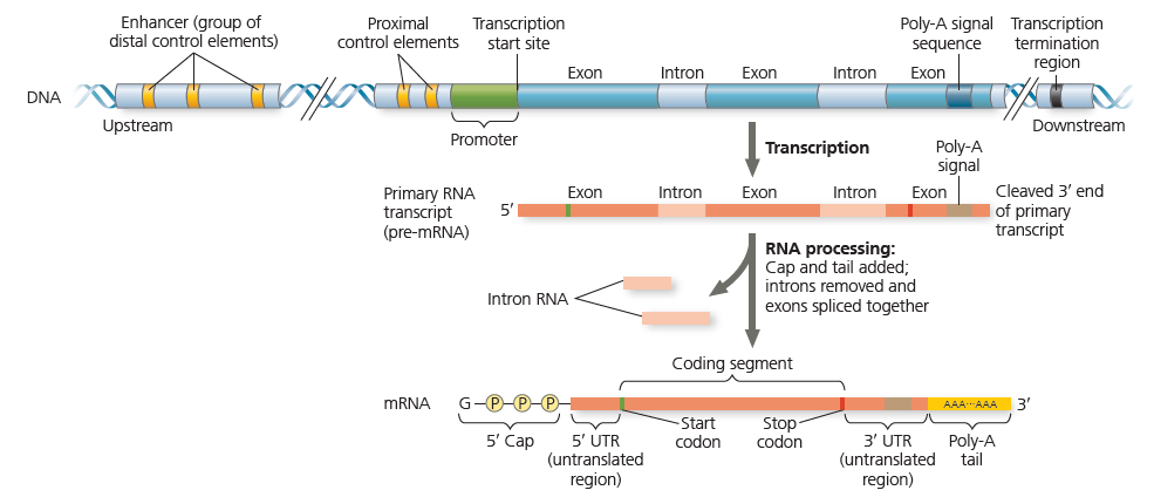
\includegraphics[width=\textwidth]{figures/from-DNA-to-RNA.png}
     \captionsetup{singlelinecheck=off}
    \caption[An eukaryotic gene and its transcript.]{
    This figure is reproduced from ~\autocite[Fig.~18.9, p.~373]{campbell_etal20}. 
    \begin{itemize}
        \item \textbf{Eukaryotic gene structure.} In addition to the coding sequence itself, each eukaryotic gene has a promoter, a DNA sequence where RNA polymerase binds and starts transcription. Control elements (in gold) \enquote{upstream} of both types, either close (proximal to) or far (distal to) from the initiation site, are involved in regulating the level of transcription. At the other end of the gene, a polyadenylation (poly-A) sequence signals roughly where the transcript is cleaved and the poly-A tail is added, while the RNA polymerase may proceed the transcription up to hundred of nucleotides further, stopping in the \emph{transcription termination region}. But the corresponding ribonucleotides are not added to the mRNA strand, and are rapidly degraded by enzymes instead.
        \item \textbf{Pre-mature RN.} Enzymes modify the two ends of a eukaryotic premRNA by the addition of the 5' cap and poly-A tail. The modified ends enable to export the mRNA to the cytoplasm, protect it from degradation and promote ribosome attachment during the protein synthesis phase. The 5' cap and poly-A tail are not translated into protein, nor are the 5' and 3' untranslated regions. The pink parts are the introns, sequences of RNA that are removed of the final mRNA strand, while the exons, the red parts, remain.
        \item \textbf{Mature mRNA.} During RNA processing, the introns are cut out and the exons spliced together. In many genes, the introns are much longer than the exons. (The UTR regions, while not coding for proteins, are considered exons because they remain in the final mRNA strand.) In the cell, some of these processes act simultaneously, addition of the 5' cap and splicing occurs while transcription is still under way.
    \end{itemize}}
    \label{fig:from-DNA-to-RNA}
\end{figure}


\subsection{Translation}
Translation is the process of synthesising a protein molecule from a RNA blueprint, driven by ribosomes (\enquote{protein complex} mixed with ribosomal RNA). It converts codons (triplets of adjacent nucleotides) of mRNA into the corresponding amino acids, the joined polypeptide sequence of them forming a protein.  

The process of translation can be divided into three main stages: initiation, elongation, and termination.
\begin{enumerate}
    \item Translation begins with the binding of the ribosome to the mRNA at \emph{the start codon} AUG, coding for methionine. Binding is facilitated by \emph{initiation factors}.
    \item The ribosome moves along the mRNA, adding amino acids to the growing polypeptide chain in the order specified by the genetic code. The \enquote{genetic code} relates the RNA sequence to the amino acid sequence in proteins: there are in total $4^3=64$ possible sequences of 3 codons, however, only 20 amino-acids prevail in nature. This implies that distinct codons code for the same protein. Each amino acid is brought to the ribosome by a transfer RNA (tRNA) molecule.
    \item Translation terminates when the ribosome reaches one of the three \enquote{stop codons}, namely UAA, UAG, and UGA, acting as the end site of the polypeptide chain. The completed protein is then released from the ribosome.
\end{enumerate}

Defects in translation can result in the synthesis of non-functional or toxic proteins, leading to various diseases and disorders. Indeed, proteins are essential, complex molecules that perform a wide range of functions in the human body, intervening directly in most of the biomechanical processes: 

\begin{enumerate}[label=(\alph*)]
\item \textbf{Structural support:} They are the essential bricks of our architecture, including tendons, bones, and skin, whilst maintaining the cell envelope. While some are inactive, others have the ability to contract, enabling the contraction of muscle fibres, such as actin and myosin.
\item \textbf{Enzymes:} Some species of proteins catalyse biochemical reactions, speeding up reactions within cells.
\item \textbf{Transport:} Some carry essential metabolites in vital fluids of the human organism, such as blood or lymph liquids. For instance, hemoglobin is in charge with the transport of oxygen in the blood towards the organs. 
\item \textbf{Cell signalling:} They convey essential signals among cells, enabling efficient communication in remote tissues. This ranges from hormones that regulate the \gls{metabolism} and control various physiological processes, such as insulin or adrenaline, to signal \gls{transduction}.
\item \textbf{Antibodies:} they intervene in the adaptive immune system by recognising and neutralising specifically foreign invaders.
\item \textbf{Storage:} Proteins such as ovalbumin are a renewed source of amino acids for building up other proteins.
\item \textbf{DNA replication and repair:} helicases and polymerases intervene in DNA replication, transcription and repair.
\end{enumerate}

Both the linear arrangement of amino acids in the protein sequence and its three-dimensional arrangement, commonly referred to as \Glspl{protein-structure}, often separated into four scales for clarity, play a crucial role to the final biological function of the protein. It is also important to note that not all proteins possess this intricate complexity, some being merely described at the single polypeptide sequence, and that modifications at any level of protein organisation can significantly affect its operational organisation, leading potentially to severe metabolic disorders. \Cref{fig:from-DNA-to-protein} illustrates the stages involved in synthesising a functional protein from a DNA sequence. 

\begin{figure}[p]
     \centering
     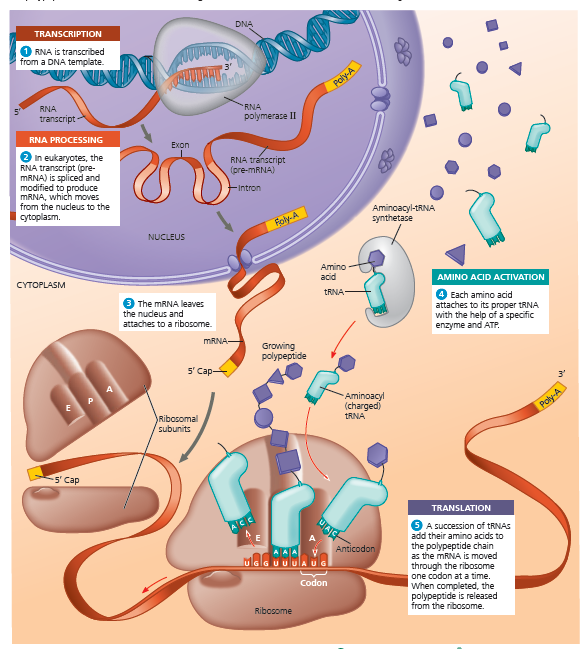
\includegraphics[width=\textwidth]{figures/from-DNA-to-protein.png}
    \caption[A schematic view of the process involved in protein production from an eukaryotic gene.]{
    This figure is reproduced from ~\autocite[Fig.~17.25, p.~356]{campbell_etal20}. Each gene in the DNA can be transcribed into several RNA molecules, and each mRNA can be translated to several proteins.}
    \label{fig:from-DNA-to-protein}
\end{figure}


\section{Regulation of gene expression}
\label{sec:gene-regulation}
\paragraph{Overview: coordinate the gene interactions:}
Just before the starting of concert, members of the orchestra individually tune their instruments in a gleeful but disordered cacophony. However, as soon as the conductor’s baton rises, all instruments join in to raise or lower their volume and their pitch at properly timing. And the original discordant sounds switch into a beautiful symphony that enraptures the audience.

In a similar way, cells must precisely regulate and coordinate their gene expression. Indeed, each cell type contains the same genetic material, however, by expressing a different subset of genes in a specific schedule, they are able to adjust to varying environmental conditions, to perform completely distinct actions, to pursue different biological roles and to fit to the growth development of the individual. Without this fine tune of gene regulation, how could we explain the complete distinct role played by a neuronal and a pancreatic cell? And how a fully developed human body emerges from a single egg cell, passing through the embryonic, foetal and adulescent stages? In the following sections we provide an overview of the \emph{regulation mechanisms} occurring in cells,  namely the way in which different genes are turned on and off at the right time. Gene regulation, as we will see, can occur in any stage of the gene expression process.

\subsection{Regulation of the chromatin structure}
Firstly, the level of transcription is modulated by the availability of the initiation sites and by extension to the level of compactness of the chromatin fibre.  Recall from \Cref{subsec:DNA}  that the DNA of eukaryotic cells is packed with proteins in a \enquote{protein complex} known as chromatin, the basic unit of which is the nucleosome. Indeed, when histones and DNA are tightly bound in the chromatin fibre, they limit the access of the RNA polymerase to promoters. This phenomenon of dynamic modification of chromatin architecture is called \emph{chromatin remodelling}.


The regulation of gene expression with respect to the compactness of the chromatin structure is influenced by three factors: the location of a gene’s promoter relative to the initiation sites, the overall compactness of the chromatin structure, for instance, genes within the heterochromatin, a highly-condensed region remain unexpressed. Lastly, some chemical modifications catalysed by specific enzymes over the tails of the histones protruding outward from nucleosomes or the DNA sequence itself can influence locally the chromatin structure by modifying the tridimensional structure and the folding of the histone proteins. 

Reversible addition of methyl groups (-CH3) to amino acids in histone tails can promote the condensation of the chromatin, while addition of a phosphate group, namely \emph{phosphorylation},  or \emph{histone acytelation}, namely when acetyl groups attach to lysines, induce a looser structure of the chromatin. The \emph{histone code} hypothesis suggests that the specific combination and order of chemical modifications yields the final configuration of the chromatin, which in turn influences transcription.


While some enzymes interact chemically with the tails of histone proteins, \emph{DNA methylation} refers to the process performed by a different set of enzymes, methylating directly certain bases in the DNA itself. It generally occurs at CpG (Cytosine-phosphate-Guanine) sites, the regions of the DNA sequence where a guanine follows a cytosine. DNA methylation mechanisms play a critical roles in gene silencing by inducing the condensation of the chromatin. Notably, DNA methylation seems to be involved in the long-term inactivation of genes supposed to remain active only during the embryonic phase. In opposition to the reversible changes induced by histone methylation, it seems that the methylation patterns remain permanent, with highly-specialised cells keeping the methylation blueprint acquired during the developmental phase, a process named \emph{genomic imprinting}. 

\todo{def eukaryotic, add illustration of the complex structure of a gene and alternative splicing, heterochromatin and eurochromatin 330-379 Campbell 12}

\subsection{Regulation of transcription initiation}
\label{subsec:reg-transcript}
Chromatin-modifying enzymes provide the first initial regulation of the
gene expression by controlling the access of a region of the DNA either more. Once the promoter site is reachable, the initiation of transcription involves the recruitment of proteins, building a \emph{transcription initiation complex} \Cref{subsec:transcript}.

Among them, the RNA polymerase II transcribes the gene and synthesises it into a primary RNA transcript (pre-mRNA). However, appropriate binding and efficient transcription requires the combination of regulatory proteins called \emph{\Glspl{tf}} with their corresponding binding sites acting as control elements.  Together, \acrshort{tf} interplay to precisely achieve the fine-tune regulation of gene expression seen, either activating or inhibiting the transcription process.


We set apart two types of transcription factors:
\begin{itemize}
    \item \emph{General transcription factors:} They are required for the initiation of the transcription of all genes, by either binding to the TATA box, a sequence present in most promoters, to other \acrshort{tf} or to RNA polymerase. However, their presence only leads to a low rate of RNA production. 
    
\item \emph{Specific transcription factors}: Precise and specific production of a given gene involves another set of proteins, the so-called specific \acrshort{tf}. They recognise specific sequences of DNA, that might be located close to the promoter (\emph{proximal control elements} or may be distant up to thousands of nucleotides upstream or downstream, the \emph{distal control elements}. A group of control elements acting together to which a TF uniquely binds to is called an \emph{enhancer}. Interestingly, while a gene may be associated to several enhancers, whose availability varies over time, each enhancer is only associated with a gene. 

\acrshort{tf} can either act as activators or repressors, and bind to other \acrshort{tf} or the DNA sequence itself. In the last case, they display the same two structural elements: a \emph{DNA-binding domain} that binds to the corresponding DNA control elements and several \emph{activation domains} that ease or inhibit \GLS{ppi} networks and by extension the efficiency of the transcription. 
\end{itemize}

Amazingly, while up to \num{20000} genes must be regulated in a human cell, only a dozen distinct nucleotide sequences control the pairing between TF and the DNA sequence, each enhancer being composed
on average of about ten control elements. It is the particular combination of control elements that yields the one-way matching between the enhancer and its corresponding TF. 


\subsection{Post-transcriptional regulation}
\label{subsec:alternative-splicing}

Recall from \Cref{subsec:transcript} that the original strand of mRNA resulting the transcription is not yet mature, and undergoes a series of biochemical interactions modifying its properties. Among them, \emph{alternative splicing} is the most fundamental mechanism of post-transcriptional regulation. 

Indeed, while all the introns are removed, not all the exons, even though coding directly for a protein, are kept in the final mature mRNA. It enables the production of protein variants, \emph{isoform proteins}, starting from the same pre-mRNA, as illustrated with the troponin gene below \Cref{fig:alternative-splicing}. Thus, a single gene can achieve different functions in the cell by controlling the proportion of each isoform produced. In fact, alternative splicing is the most likely explanation until now ($90\%$ of human protein-coding genes undergo splicing) for the low number of human genes identified (around \num{20000}), similar to that of a soil worm (nematode) or a mustard plant. 

\begin{figure}
    \centering
    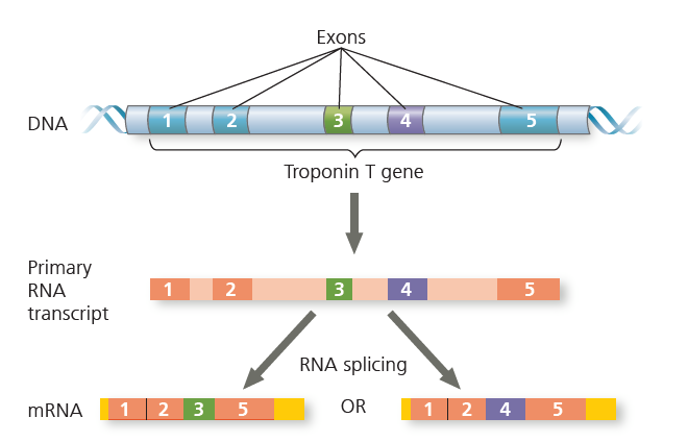
\includegraphics{figures/alternative-splicing.png}
    \caption[Alternative RNA splicing of the troponin T gene.]{This figure is reproduced from ~\autocite[Fig.~18.14, p.~378]{campbell_etal20}. Colour background of the exons are dark and introns light. The primary transcript of this gene can be spliced in several mRNA strands:  one ended up with exon 3 (in green) and the other with exon 4 (in purple). Both mRNAs are muscle proteins, differing slightly by their operational region.}
    \label{fig:alternative-splicing}
\end{figure}
Once the mature mRNA produced, it still must be translated into a protein. Conversion from a mRNA fragement to a functional protein highly depends on its average life span, which in return is related to the presence of translation regulatory proteins that recognise sequences of the 3 or 5' UTR(specific inhibition control, by preventing the binding of both RNA ends to the ribosome) or general effect protein factors, notably involved in development and differential phase. We display the mechanisms involved in ~\Cref{fig:model-enhancer}.

\begin{figure}
    \centering
    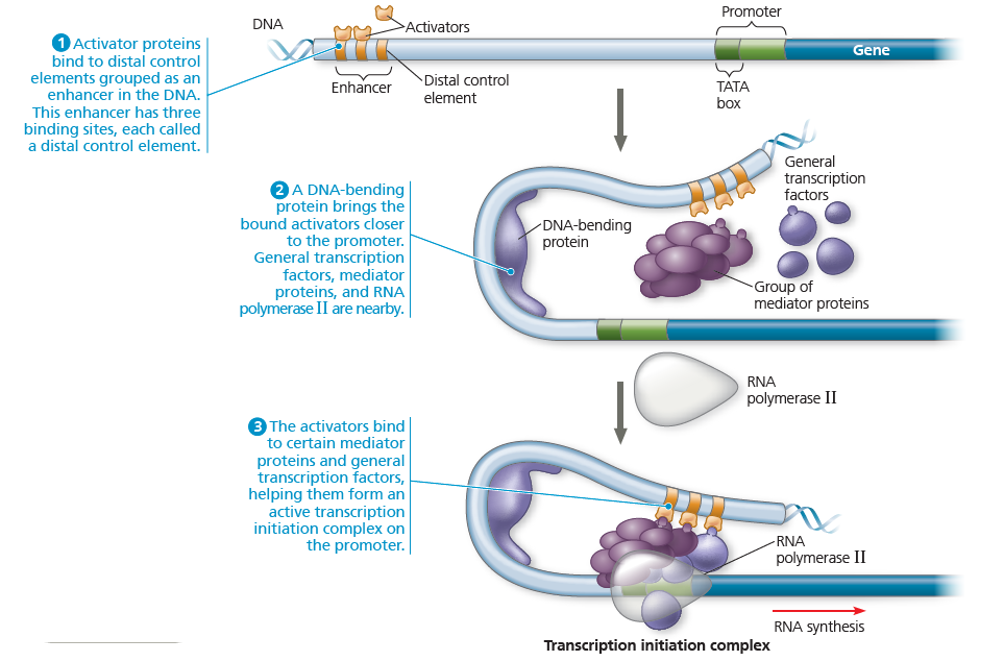
\includegraphics{figures/model-enhancer.png}
    \caption[\textbf{Model for the coordinate action of RNA polymerase and \acrshort{tf}.}]{This figure is reproduced from ~\autocite[Fig.~18.11, p.~375]{campbell_etal20}. The transcription initiation complex involves the coordinate binding of RNA polymerase II and general transcription factors, while fine-tune regulation is enabled by specific \acrshort{tf} that bind to the enhancers (here, represented with three control elements in gold) and to mediator proteins. It is DNA bending that enables enhancers to influence the regulation remotely. }
    \label{fig:model-enhancer}
\end{figure}


Interestingly, recent researches highlight the combined role of small non-coding RNAs (ncRNAs) molecules, known as microRNAs or miRNAs, and regulatory proteins in modulating gene activity. By base pairing to mRNAs, microRNAs mediate translational repression or the degradation of mRNAs. Other non-coding RNAs, including long intergenic ncRNAs (lincRNAs) or small interfering RNAs (siRNAs), seems to be involved but the associated regulation mechanism still needs to be deciphered. 

One of the first worldwide initiative related, to decipher the whole genome, is the ENCODE (Encyclopedia of DNA Elements) project, initiated in 2003: the main objective was to link a significant portion of the human genome to biological functions, encompassing protein-coding and non-coding genes. Another aspect of the program involved examining the associations between DNA sequence and histone tridimensional structures that influence the regulation of the gene expression(known as \enquote{epigenetic} alterations that impact gene expression while leaving the nucleotide sequence unaltered).Notably, this second phase involved more than 440 scientists in 32 research groups and 1,600 curated genomic experiences, and confirmed the high biological relevance of miRNAs while mitigating the wrongly acknowledged statement that most of the human genome was just \enquote{junk DNA}. Indeed, biochemical functions have been assigned to at least $80\%$ of the genome, $75\%$ of the human genome was found transcribed into functional RNA at some point whereas less than $2\%$ actually codes for proteins (\autocite{desouza12}, \autocite{ecker_etal12}, \autocite{gerstein_etal07} and \autocite{snyder_etal20}).


Complex biological functions require a coordinate set of chemical reactions, each with its own associated proteins, for instance the enzymes involved in a metabolic pathway or a transduction signal. As opposed to the solution developed in bacteria, in which genes involved in the same biological function are associated to the same promoter (\emph{operon} structure), genes that require co-expression are often scattered over the whole genome in human cells. In that case, coordinate control is triggered by \gls{cellular communication}, that in turn promote the recruitment of \acrshort{tf}. Since they move freely in the nucleus,  they are able to recognise and bind to the whole set of control elements.



\subsection{Post-translational regulation}
\label{subsec:post-transla}
Finally, post-translational modifications can occur at any time after the translation of the protein. By inducing chemical modifications to proteins, they alter its metabolic function or \emph{targeting}, a part of the protein sequence itself that addresses the final polypeptide sequence to its appropriate localisation. The most common modifications involve covalent additions of one or more side groups, including without intention of exhaustivity, phosphorylation, acylation, alkylation, and glycosylation. 

For instance, cell-surface proteins require membrane targeting and addition of sugars to get functional, while the insulin polypeptide proceeds from an original bigger precursor. 

Finally, the life span of each protein is strictly regulated by selective degradation. Giant protein complexes, the \emph{proteasomes}, recognise the ubiquitin-tagged proteins and degrade them. 


The several modifications discussed before do not entail a change in the DNA sequence, yet they may be transmitted to future generations of cells. The mechanisms involved in the inheritance of these specific traits is called \emph{epigenetic inheritance}, which in opposition to DNA mutations, are generally reversible. An increasing number of experiences confirm the importance of epigenetic may explain why only one of a pair of twins develops a genetically-based disease or the initiation of pro-tumoral conditions promoting the apparition of cancers. 

The control the epigenetic regulation mechanisms is itself modulated by the interactions between genes and the environment. Indeed, the degree of DNA methylation is thought to be related to the availability of nutrients. We display below a diagram summing up the biological mechanisms involved in gene regulation \Cref{fig:gene-regulation}.

\begin{figure}
    \centering
    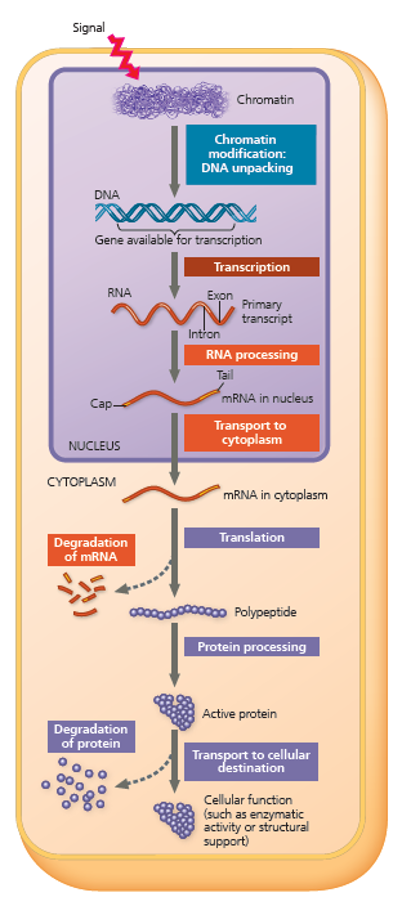
\includegraphics{figures/global-gene-regulation.png}
    \caption[The main gene regulation stages.]{This figure is reproduced from ~\autocite[Fig.~18.6, p.~370]{campbell_etal20}. In this diagram, each colour indicates the type of molecule regulated (blue = DNA, red or orange = RNA, purple = protein). Not all genes are regulated at all stages.}
    \label{fig:gene-regulation}
\end{figure}

\todo{autre figure, ou en GRN, à mettre ici, du stage de boolean}

It's worth noting that the entire regulatory machinery might not always be involved in the regulation of the production of specific gene. Furthermore, certain regulatory factors can operate on multiple levels: \acrfull{tf} can influence chromatin structure indirectly by recruiting proteins that acetylate histones to enhance transcription or directly by removing acetyl groups, resulting in transcriptional \emph{silencing} ~\autocite{walters_etal12}. More recently, new \emph{chromosome conformation capture} techniques reveal that entire regions within a chromosome (\emph{topologically associated domains}, or \emph{TADs}) bind into loops and congregate with each other, or with TADs from other chromosomes, to form sites associated with high transcriptional activity levels and often related to a given biological function. These \emph{transcription factories} are indeed rich in RNA polymerase and other \acrshort{tf}. 

In next section, we detail some sequencing tools that can be used to keep track of the variations of the transcriptome and help unravel the relations between the biological features. 

\section{Capture variations of the transcriptome}
\subsection{Overview: definition of the transcriptome:} 
\label{subsec:transcriptome-overview}
Among the several types of omics that can be analysed to unravel the relationships between the biological entities, wefocus on transcriptomics, the analytical study of the transcriptome, as it is certainly the kind of biological data for which the most technologies have been developed, and as it indirectly provide clues on the interaction between DNA and protein and how they contribute to the biochemical processes involved in keeping the organism in proper operating order. The transcriptome is simply the collection of all RNA molecules, types and quantity, present at a given time in a biological sample.  

While tools for quantifying gene expression levels have been developed for years, for a long time, they focused on a single gene at a time. Among them, the most widely used were Northern blots or Reverse Transcription-Polymerase Chain Reaction (\acrshort{rtpcr}) as well as sequence-based approaches such as Serial Analysis of Gene Expression (SAGE) or comparative Expressed Sequence Tag (EST). Nevertheless, all the technologies described above have in common the generation of a sequence of nucleotides complementary to the original material. Precisely, the specific mRNA sequence of interest is used as a template to synthesise a complementary, single-stranded RNA strand using nucleic acid hybridisation (recall from \Cref{subsec:DNA} that the two strands of DNA hold from base-pairing, with each nucleotide uniquely recognising another amino acid among a repertoire of four, property called \emph{hybridisation}). Each of these paired nucleotides, used as as a surrogate for the presence of the mRNA, is called a \emph{nucleic acid probe}. In addition, the pair original mRNA-cRNA or DNA is uniquely identified with a fluorescent tag, in a technique called \emph{in situ (\enquote{in place}) hybridisation.} (the total number of mRNAs that can be followed at the same time is however limited). 


As an example, we describe in few words the widely used \emph{reverse transcriptase polymerase chain reaction (\acrshort{rtpcr})} method. The first step consists of synthesising a double strand complementary DNA sequence, expunged of introns, by the combined use of reverse transcriptase and DNA polymerase with a RNAse enzyme in charge of degrading the original mRNA material. Indeed, RNA is reverse transcribed to cDNA since DNA is more stable and enables more efficient amplification and the use of mature DNA sequencing technology. Then follows an \emph{amplification stage} generating many copies of the RNA segment of interest: the PCR step, which notably requires \emph{primers}, short chemically synthesised oligonucleotides that initiate the replication by attaching the DNA polymerase in place. Finally, newer methods such as qRT-PCR (\emph{q} stands for \emph{quantitative}) enable precise quantification while avoiding the burdensome and time-consuming electrophoresis step.


However, it is generally much more interesting to capture \emph{simultaneously} the evolution of the mRNA levels between all the genes to better understand how they act in concert to perform complex biological functions. This new approach of the field is called the \emph{systematic approach}. For that reason, we focus on the technologies that enable to analyse the \emph{whole transcriptome} in a high-throughput manner, with, by chronological order, the apparition of microarray technologies, and then the development of Next-Generation Sequencing (\acrshort{ngs}) methods. Compared to microarray, \acrshort{ngs} technologies present the main advantage of not being restricted to already known documented DNA or RNA sequences. 

The principle and technology of microarrays and RNASeq methods are further detailed respectively in \Cref{subsec:microarray} and \Cref{subsec:RNASeq} from a molecular biologist and \gls{bioinformatic} point of view, namely from the data production workflow to the raw mapping of counts, without further normalisation. Promising technologies, that would enable to follow in real time the spatial and temporal evolution of transcriptomics, are mentioned in the last paragraph of this section \Cref{subsec:miscelleanous-innovative-rna-seq}. Note that these promising technologies would not have been possible without the global sequencing projects in late $20^\text{th}$ century, as most of them rely on a reference genome to align the investigated mRNAs. 

Finally, once we have collected the raw counts or arbitrary quantitative units (for microarray), we detail statistical methods in \Cref{chap:transcriptome-workflow} to address the challenges associated with this type of data, along with appropriate normalisation processes to apply these method. Transcriptome datasets find diverse biological applications, including \emph{differential analysis}, which aims to identify genes exhibiting significant differential expression between two distinct biological conditions (often involving comparisons between control/healthy and disease samples),  subgroup identification of patients sharing similar expression profiles, usually by performing \emph{clustering}-based methods and computation of the disease prognosis. These methods typically operate within a semi-supervised framework, often integrating prior medical knowledge with \emph{unsupervised} machine-learning techniques.


 \subsection{Microarray technology to quantify gene expression}
\label{subsec:microarray}
Microarray plates are small chips onto which tens of thousands oligonucleotide probes, with sequences complementary to fragments of actual genes, are engraved. Generally, each gene is normally represented by a set of probes, so called a \emph{probeset}, each representing a different but highly-specific gene region. Indeed, designing customised probes reveals a painstaking task, as the challenge is to identify a combination of nucleotides both characteristic of our coding gene and not matching any other genome region, with the risk of detecting a spurious pairing otherwise. In addition, due to natural limitations of sequencing technologies, the length of the complementary probe is thus generally between 25 bp and 60 bp long.  

The following protocol is common to most of the microarray technologies:
\begin{enumerate}
    \item The mRNA samples, called the \enquote{targets}, are extracted from the investigated biological sample. 
    \item The targets hybridise to their complementary probe on the microarray and are labelled using fluorescence or radioactive labels. 
    \item Two competitive methods are used to compare gene expression levels between two biological conditions, as presented in \Cref{subfig:one-vs-two-channel}. Either the two mRNA preparations are hybridised at the same time, the RNA strands competing for the access to the probes, or each sample is assigned its own array, but with the same dying label (an extensive comparison of the pros and perks of both approaches is reviewed in \autocite{patterson_etal06}, \autocite{kuo_etal06}, \autocite{severgnini_etal06} and \autocite{sirbu_etal12}). In both cases, each probe is generally duplicated thousands of time in the same \enquote{probe cell} (see \Cref{subfig:probe-structure} for details), called a \emph{spot}, to trap the target mRNA fragment.
    \item Once the hybridisation step is performed, high-spatial resolution pictures of the plate are carried out, on which a spot is likely to be represented by many pixels. The \emph{segmentation} stage sets apart pixels proceeding from a spot, marked as relevant signal, from pixels out, marked as background noise. Finally, the \emph{quantification} stage itself aggregates the individual intensity values of a spot into an unique signal, used as proxy of the abundance of mRNA and reports them in files with CEL extension.
\end{enumerate}

\begin{figure}
     \centering
     \begin{subfigure}[p]{0.2\textwidth}
         \centering
         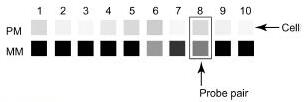
\includegraphics[width=\textwidth]{figures/biological_introduction/probe_structure.jpg}
         \label{subfig:probe-structure}
         \caption[\textbf{Probe set structure}]{A micro-array chip is composed of a huge collection of probe oligonucleotides whose sequence is complementary to RNA targets. 
         To enhance detection power and assess variability, the probes are further organised into \textit{probe sets}:  a collection of perfect match probes (PM) that precisely match the target sequence paired with mismatch probes (MM) that only differ by a single base mismatch.
         Hereby, we can assert the specificity of each probe by quantifying the relative binding of the target sequence between the PM and MM probe. 
         The collection of probes is stored in a CDF file and the related value in a CEL file, each of them being uniquely identified by an affyID, figure reproduced from \href{https://www.affymetrix.com/support/downloads/manuals/chas_2_1_user_manual.pdf}{Affymetrix technical manual}.}
     \end{subfigure}
     \hfill
     \begin{subfigure}[p]{0.55\textwidth}
         \centering
         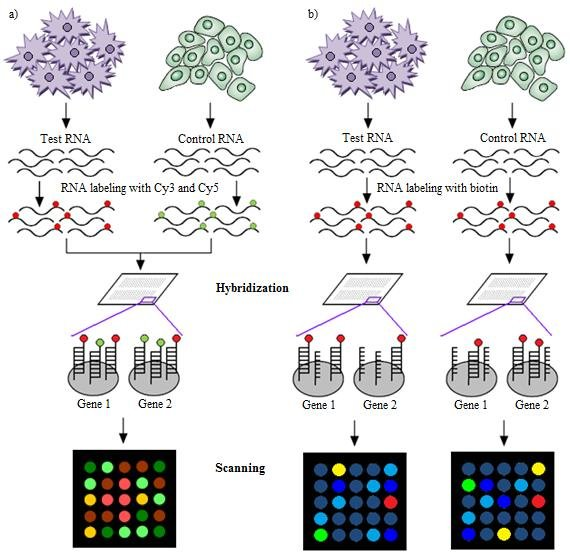
\includegraphics[width=\textwidth]{figures/biological_introduction/Microarray-Hybridization-using-a-two-channel-and-b-single-channel-microarray.png}
         \label{subfig:one-vs-two-channel}
         \caption[\textbf{a) Two-channel and b) Single-channel microarray platforms}]{This infographic (reproduced from \autocite[Fig. 6]{dawany23}) illustrates the technical protocol differences between single-channel and two-channel microarray technologies. Briefly, one-colour channel Microarray uses a single fluorophore to quantify the relative signal intensity of a disease sample against a common reference (generally a control, healthy case-control) and exhibits simpler experimental design. On the contrary, two-colour channel Microarray methodology is based on two different fluorophores (often Cy3 and Cy5) to compare directly two samples within the same microarray slide, hereby offering enhanced sensitivity to detect differential gene expression in comparative analyses.}
     \end{subfigure}
   \caption[A brief overview of micro-array chips to quantify the transcriptome]{}
    \label{fig:microarray-technology}
\end{figure}

Although generally neglected nowadays against \acrshort{ngs} technologies, new promising microarray applications continue to emerge, ranging from \acrshort{snp} detection to copy number variations through identification of methylated regions or protein binding sites. Notably, their extreme high miniaturisation makes them the best compromise between the requirement of high-throughput and cost-saving technologies, one of the most widely used technology being the \href{https://www.affymetrix.com/support/downloads/manuals/chas_2_1_user_manual.pdf}{Affymetrix} suite \footnote{For instance, the Human Genome U133 Plus 2.0 Array (HGu133+, released by the Affymetrix company) gathers \num{54000} probesets, spotted by 11 different probes, comprising overall more than \num{1300000} distinct oligonucleotide sites.}, with a bunch of dedicated R packages and methods to aggregate probesets into an unique gene expression measure while discarding background noise or accounting for specific bias (\autocite{gautier_etal04}, \autocite{irizarry_etal03}).


\subsection{RNASeq technology}
\label{subsec:RNASeq}
\acrfull{ngs} methods are cutting-edge technologies, emerging from early 2000's, that bridge the gap between the high-throughput sequencing capacity of microarray technologies and the versatility of traditional sequencing methods which can build from scratch an unknown genome. Numerous sequencing methods have been developed, with different biological applications and limitations. We generally identify three sequencing generations, differing by the nature of the reads generated (either short or long, direct RN or requiring prior conversion to cDNA) and the sequencing throughput.


First-gen(eration) \glspl{sequencer}, like the ABI capillary technology, offer high accuracy and longer read lengths, but lack high-throughput sequencing. Second-gen platforms (e.g., Illumina's MiSeq, HiSeq, NextSeq and Thermo Fisher Scientific's Ion Torrent) achieve both high throughput and accurate \emph{base-calling} via parallel sequencing. However, their shorter read lengths pose challenges in assembling repetitive sequences. In contrast, third-gen sequencers (e.g., Pacific Biosciences' PacBio, Oxford Nanopore Technologies' MinION, PromethION, SmidgION) generate long reads at high throughput by sequencing single-molecule, at the expense of a higher error rate. In this section, we focus on the Illumina sequencing technology since all the datasets used for our analysis were sequenced through this platform \footnote{Going further,it is up to $90\%$ of all DNA sequenced data that were generated with the Illumina platform, from estimations reported in \href{https://emea.illumina.com/techniques/sequencing/rna-sequencing/total-rna-seq.html}{Illumina leaflet}, in 2015.}, which is not surprising since the human genome is well annotated and we were only interested in our downstream analyses in comparing transcriptomic profiles at the gene level, not the isoform one, across thousands of biological samples. However, the interested reader may report to glossary keys \glspl{sequencer} for a comprehensive review of sequencing techniques and \glspl{library} for an overview of biological applications with respect to the nature of the generated reads. \autocite{slatko_etal18} describes generation after generation the mere principles underlying each technological breakthrough along with a collection of useful papers and web links for each sequencing platform, and \autocite{vilgis_deigner18} is a book chapter addressed specifically for practitioners of precision medicine. Ultimately, \autocite{lam_etal12} and \autocite{cottrell18} are essays reviewing quantitatively several RNASeq methods, while proposing further possible evolution perspectives for these technologies.


Hence, while the final choice of the sequencing platform choice depends on the biological application and the human expertise and financial resources available, all of them present the following four stages in their workflow sequencing pipeline, summarised in \Cref{fig:rna-seq-workflow}:

\begin{enumerate}[label=(\roman*)]
    \item \textbf{Library preparation:} The transcriptome of the sample or tissue of interest, after an isolation stage, is reverse-transcribed into \gls{cDNA} for stability purposes. The next step consists of randomly fragmenting cDNA into strands of smaller sizes, called \emph{inserts}, and ligating two distinct adaptors, one at each end, in a process called \enquote{tagmentation}. The set of obtained cDNA fragments is termed the \enquote{library} (see also subfigure a, in \Cref{fig:rna-seq-workflow}).
    
    \item \textbf{DNA amplification:} Compared to old-fashioned sequencing methods, \acrshort{ngs} technologies mostly differ by their higher capacity of DNA amplification and sequencing. After an initial amplification stage, employing similar techniques to \acrfull{rtpcr}, comes the \emph{clonal amplification} stage itself in order to increase by several orders of magnitude the total amount of DNA available for sequencing, compared to more traditional approaches (note that this prior amplification stage is mostly required for sequencing methods that do not sequence directly RNASeq, but rather convert it first into cDNA, as reviewed in \Cref{subfig:library-comparison-preparation}). Here, the DNA amplification process largely differs between platforms, thus we restrain to the study of the \Gls{illumina} protocol. Precisely, the clonal amplification stage mitigates the lower sequencing quality inherent to \acrshort{ngs} in comparison to conventional methods, while achieving a significantly stronger genome coverage \footnote{Up to 180 million reads are generated by the HiSeq 2000 platform}. This is particularly valuable for sequencing challenging regions of the genome, including repetitive segments, GC-rich regions and \emph{homopolymers}, which tend to pose accuracy hurdles during sequencing.
    
    The initial Illumina amplification relies on a lawn of oligonucleotides, complementary to the sequences of the adaptors, which are attached to a glass surface, called a \emph{flow cell} and composed of thousands of \emph{tiles}. In parallel, the DNA library is \emph{denatured} to form single-stranded DNA (ssDNA) fragments which subsequently tether to the surface-bound oligonucleotides.
     Next, the so-called amplification stage relies on a process called \enquote{bridge amplification}, in which each hybridised fragment is cloned separately and simultaneously into $\approx 1000$ copies, forming a \emph{cluster}. This process is enabled by the two types of oligonucleotides bound to the flow cell: they indeed allow alternated synthesis in both directions of the cDNA fragments, a process repeated until the desired amount of DNA has been reached (see also subfigure b, in \Cref{fig:rna-seq-workflow}). 
    
    \item \textbf{Sequencing:} Genome sequencing consist of determining the sequence of nucleotides of the whole set of fragments composing the DNA library and the technique is itself highly dependant on the platform used. The resulting data output is typically stored in \Gls{FASTA} or FASTQ files.
    
    Again, we focus on the Illumina high-throughput and massively parallel sequencing protocol. Briefly, fast sequencing of fragments rely on a proprietary reversible \enquote{terminator} method that detects single addition of bases in the mean time they are incorporated. Specifically, each sequencing cycle starts with the addition of a primer and fluorescent reversible-terminator nucleotide (rt-dNTPs), ensuring that only one nucleotide is added at a time. Any unbound nucleotide is then washed away, while lasers excite the fluorescent tags of each incorporated nucleotide, each being associated to its own wavelength. Finally, the tag is cleaved off, putting an end to the cycle. This procedure, known as \enquote{sequencing-by-synthesis} is iteratively performed until the desired sequence length is achieved. The number of cycles employed dictates the resulting sequence length, a balanced trade-off between generating overly brief strands that might yield ambiguous mapping information in the subsequent assembly stage, and overly extended ones that carry an elevated risk of compromised synthesis quality at the 3' end. 
    The resulting images are then processed to return the \emph{reads} themselves (the string sequence, each character coding for one of the four RNA nucleotides). To achieve this, the nucleotide identification process computes the signal intensity and noise for each of the identified cluster, in every set of raw image files generated during the \enquote{sequencing-by-synthesis} phase. This transformation of raw intensities into interpretable reads encompasses tasks such as background noise correction, accurate cluster identification, and determination of scaling intensity. This multifaceted procedure is referred to as \emph{base-calling} (see also \autocite{illumina23} for an industrial overview or \autocite{raghavendra_pullaiah18} and \autocite{meyer_kircher10} for a didactic and unbiased academic point of view).
    Better sequencing quality can be further achieved by synthesising fragments in both directions of each cDNA sequence, as illustrated in \autocite[Figure 4: Paired End Sequencing]{illumina23}. The resulting \enquote{paired-end} library has twice the number of reads for the same dedicated efforts, increasing the quality of the alignment and providing refined opportunities for the detection of \enquote{indels} (insertion deletion modifications), \acrshort{snv} and \acrshort{snp} mutations (see also subfigure c, in \Cref{fig:rna-seq-workflow}).        
    
    \item \textbf{Alignment and assembly:}  From the billions of reads sequenced, computer software and bioinformatic tools rebuild the whole transcriptome, by locating each read in the genome. Two strategies are used, depending on the level of prior information available: \emph{de-novo} strategy, as its name suggests, refers to construction of genomes when no annotations are available while the \emph{genome-guided} strategy aligns and maps reads onto a genome of reference.     
    \emph{De-novo alignment} is a highly-challenging task, especially for covering highly repetitive regions of the genome, while early errors performed at this stage can drastically reduce the performance of downstream analyses, notably the methods targeting genomic events, such as chromosomic rearrangements, \acrfull{snp} or even indels (for inserts and deletions). However, such issues can be alleviated by coupling short-read assembly with long-read paired-end sequencing information. This strategy, known as \glspl{genomic-scaffolding} involves generally an intermediate step which consists of generating larger individual \glspl{contig} before the final reconstruction of the whole genome. And \autocite{luo_etal21} (a comprehensive state-of-the-art review of scaffolding methods in genome assembly), \autocite{rice_green19} and \autocite{sohn_nam18} (provides guidelines for determining the optimal approach based on input data and computational budget, providing an optimised use from long reads to overcome the limitations of short reads) established that the optimal sequencing quality and coverage are achieved by combining reads of diverse sizes: shorter ones derived from \acrshort{ngs} and longer inserts obtained through traditional sequencing methods, generally with lower read depth.
    
    We now focus on the \emph{reference-based strategy}, generally favoured for human genome assembly since it has already been reconstructed globally in the early 2000's. While historically, the literature corpus focused on alignment methods for long reads generated through conventional sequencing, such as the renowned BLAST \autocite{altschul_etal90},  such methods are unsuitable for aligning the short reads returned by \acrshort{ngs} technologies nor pairing fragmented and discontinuous RNA fragments (remember from \Cref{subsec:transcript} that certain parts of the original DNA sequence are discarded in mature mRNA, including all \emph{introns}, or split into several parts). Lastly, short reads with repetitive patterns have an equal chance of aligning to various distant regions of the genome, as discussed in \autocite{treangen_salzberg12}.
     Hence, numerous alignment bioinformatic tools, designed specifically to address this short-sized issue and review in \autocite{treangen_salzberg12}, have been developed since then. Notably, to deal with alternative splicing (\Cref{subsec:alternative-splicing}), most of these methods proceed shorter portions of the read, named \endquote{seeds}, through dynamic programming, in order to find the alignment with the most overlapping sequences (among developed mapping algorithms, the most popular are BowTie2 \autocite{langmead_salzberg12}, TopHat2 \autocite{kim_etal13}, STAR \autocite{dobin_etal13} and HISAT2 \autocite{kim_etal19}). The final output is a BAM file, which can be interpreted as a global map of the genome, in which each read is associated a unique pair of \enquote{genomic spatial coordinates}. We also denote the final number of reads identified and mapped to the genome as the \emph{library size} or \emph{sequencing depth} (see also subfigure d, in \Cref{fig:rna-seq-workflow}).  
     
     \autocite{srivastava_etal20} benchmarks a huge collection of alignment and mapping methods to determine their impact on the estimation of transcript abundance estimation. They observe significantly different and variable performance between lightweight-mapping and more traditional alignment-based methods. They tried to elucidate this diversity by examining a bench of factors, and observe notably that performing spliced alignment to the genome and then projecting these alignments to transcriptome provides better mapping performance compared to directly aligning to the transcriptome.
    
    \item \textbf{Quantification:} Once all reads are aligned to a reference genome, the final stage of the RNA-seq processing workflows involves the estimation of transcript abundances, generally under the form of raw count measures at the gene or transcript isoform level. Primarily, only the reads overlapping perfectly a given exon of the original genome sequence were annotated, for instance consider HTSeq \autocite{anders_etal15} and FeatureCounts \autocite{liao_etal14} tools. Since then, advanced methods that are particularly effective with limited annotation information involve a preliminary construction of \glspl{contig}, enabling to rebuild from scratch newly unobserved transcript variants by including junction reads and unannotated transcripts (see for instance Cufflinks \autocite{trapnell_etal10} or StringTie \autocite{pertea_etal15} tools). Ultimately, Kallisto \autocite{bray_etal16} and Salmon \autocite{patro_etal17}, an updated version that accounts for sample-specific technical bias such as fragment GC-content or positional bias, are both lightweight methods relying both on a probabilistic framework and the identification of \glspl{kmer} regions, to make the alignment methods more scalable and accurate. Hence, they both stand out as cutting-edge methodologies by achieving similar accuracy to predecessors while being significantly faster (around 2 orders of magnitude, see also \href{https://gencore.bio.nyu.edu/salmon-kallisto-rapid-transcript-quantification-for-rna-seq-data}{Salmon and Kallisto: Rapid Transcript Quantification} for a practical implementation through R programming).
    
\end{enumerate}

\begin{figure}[p]
     \centering
     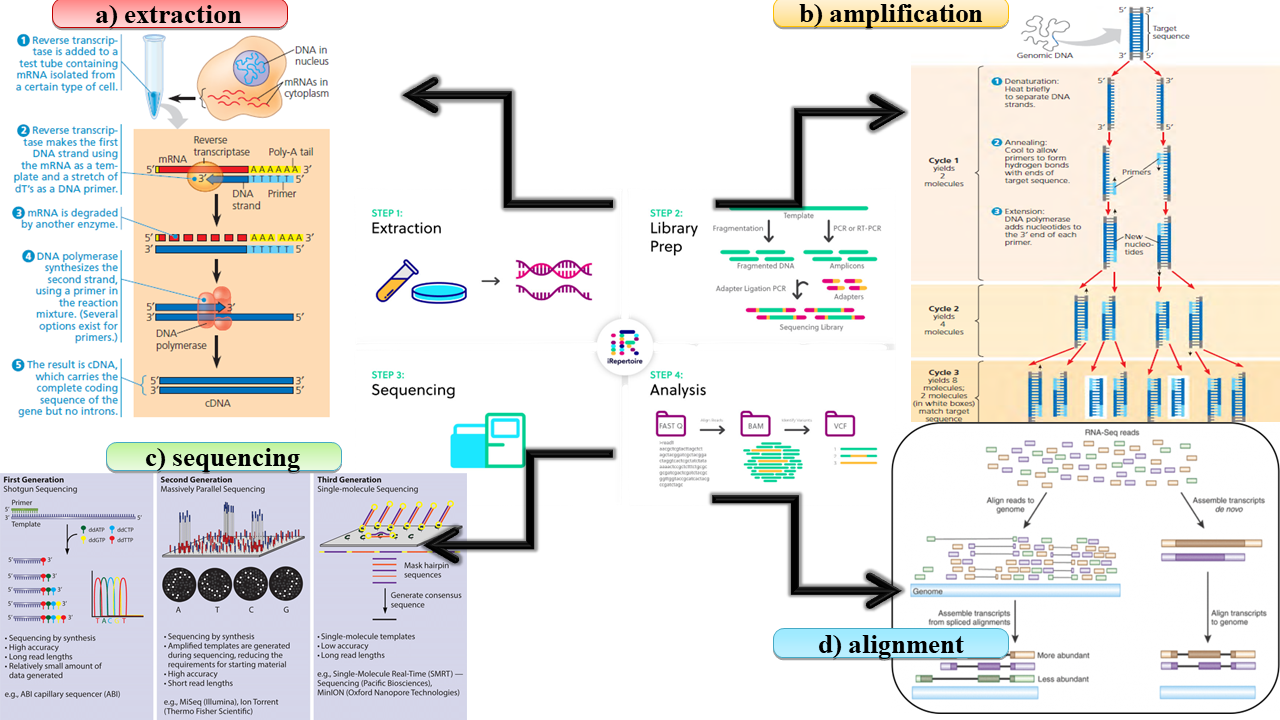
\includegraphics[width=0.95\textwidth]{figures/biological_introduction/general_workflow_pipeline.png}
     
   \caption[\textbf{Next generation sequencing (NGS) workflow:}]{
   The entire NGS workflow can be broken down into four steps: 
   \begin{enumerate}[label=\emph{\alph*})]
       \item \textit{Sample extraction:} When RNA is the starting template, an additional step, between the RNA extraction, and the library preparation itself, is required to convert the RNA into c(omplementary)DNA by reverse transcription (reproduced from \autocite[Fig 20.10]{campbell_etal20}).
       \item \textit{Library preparation:} Preparation of a sequencing library typically involves two steps: 1) \textit{RNA amplification} to increase the amount of appropriately sized target sequences and 2) the addition of \textit{adapters} to uniquely identify them. PCR (for polymerase chain reaction) is one of these techniques to copy many times any target
       sequence within a test tube, which only requires double-stranded DNA containing the target
sequence, a heat-resistant DNA polymerase, all four nucleotides, and two single DNA strands that serve as primers, one for each end of the target sequence (reproduced from \autocite[Fig 20.7]{campbell_etal20}).
       \item \textit{Sequencing RNA library:} Currently, we generally classify all sequencing platforms into three generations, each coming with distinct strengths and weaknesses (subfigure c reproduced from \autocite[Fig .1]{ronholm_etal16}).
       \item \textit{RNASeq analysis: } when studying an organism with a reference genome, it is possible to directly map the reads onto the reference transcriptome \footnotemark{1}. However, without a reference organism, the individual genome must be constructed from scratch: \enquote{de-novo assembly}, see key \gls{contig} and \gls{genomic-scaffolding} for details (subfigure d reproduced from \autocite[Fig. 1]{ronholm_etal16}).
   \end{enumerate}   
   The general framework of this illustration is reproduced from \autocite[Fig. 1]{g20}.}
    \label{fig:rna-seq-workflow}
\end{figure}

\footnotetext{Mapping reads directly to the genome presents the fundamental advantage of not knowing the exact way exons are spliced, hereby allowing the discovery of unknown variant transcripts issued from alternative splicing (see \Cref{subsec:reg-transcript}.}


The final quantification stage is used in a number of downstream analyses (see \Cref{sec:downstream-analyses}) to study dysregulated biological mechanisms and retrieve biomarkers characteristic of diseases, and may be used as well as proxy of the proteomic level, although much precaution is required due to post-transcriptional events, see \Cref{subsec:post-transla}, \Cref{sec:patrimony-overview} and paper \autocite{meissner_etal13} for limitations of RNASeq use as an intermediate measure for the proteome). 
In addition, while RNASeq enables to consistently compare ratios of transcript levels across two biological conditions sampled with the same sequencing platform, even raw counts do not correspond exactly to the absolute levels of gene expression, since this value depends on the sequencing depth (see \textbf{alignment} bullet point before), an issue partially mitigated with \Glspl{spike-in} normalisation (consider for instance the R implementation of a spike-in normalisation technique in Bioconductor package \texttt{BRGenomics} \autocite{deberardine23}.


Overall, various factors justify the increasingly prevalence of RNA-seq based technologies over microarray ones. Firstly, it does not rely on hybridization with a labelled probe, hence an annotated or reference genome is not anymore a prerequisite \autocite{wang_etal09}. Hence, relying solely on the transcripts bound to the array chips, Microarrays require good annotation for the model organism’s transcriptome, and can not capture genomic or transcriptomic individual events, such as mutated RNA or unknown alternative spliced transcript, since the mutated sequence differs from its complementary probe and hereby, is likely not to bind to it. Secondly, it can cover expression levels over a much broader range: while microarray technologies provide a continuous signal with limited detection range (background noise for low expression levels and saturation at the high end), RNA-seq inherently provides discretised measurements, quantifying gene expression as non-negative integer counts \autocite{wilhelm_landry09}. Thirdly, the versatility of RNA-seq technologies opens up new research areas, including the detection of alternative splicing isoforms and specific mutation disorders, from standard to \acrshort{snp} to more delicate general transcript fusion events \autocite{mantione_etal14} (specific benchmarking of RNA-seq based technologies, relying on concordance correlation with RT-qPCR expression data, is proposed in \autocite{everaert_etal17}. 

Precisely, \autocite{guo_etal13} observed that low abundant genes had poorer correlations between microarray and RNAseq data compared to high abundance genes, especially the Agilent two-channel microarray, with Spearman correlation of only 0.2 in TCGA datasets. Interestingly, \autocite{zhang_etal15} shows that RNA-seq outperformed microarrays in determining the transcriptomic characteristics of cancer (the studied cohort included 498 neuroblastoma patients), while both models performed similarly in clinical endpoint prediction (see also  \autocite{xu_etal13} for a more limited benchmark study comparing solely Illumina RNA-Seq and Affymetrix microarray platforms' performance). Confirming empirically these specific clinical examples, the meta-review \autocite{malone_oliver11} and opinion paper \autocite{mantione_etal14} confirm the utility of microarrays, notably as being more cost-effective and reliable for gene expression profiling in model organisms; yet, both approaches exhibit a strong congruence when asked the same biological question. 
Going further, \Cref{subsec:miscelleanous-innovative-rna-seq} summarises new RNA-Seq perspectives, notably to examine intricate transcriptome fine structure, such as allele-specific expression and isoform identification.

\subsection{Perspectives: single cell and spatial transcriptomics}
\label{subsec:single-cell-spatial-transcript}


\paragraph{Limitations of \acrshort{RNA-Seq} technologies}

As reviewed in \Cref{subsec:miscelleanous-innovative-rna-seq} and \Cref{subsec:RNA-Seq}, the ability of \acrshort{RNA-Seq} technologies to perform high-throughput sequencing analysis and sample multiplexing gives new insights on biological mechanisms. However, they are tailored to dissect bulk mixtures mixing different biological entities, preventing from deciphering complex biological mechanisms proceeding from interactions between distinct biological entities. Additionally, \acrshort{RNA-Seq} outcomes are simply snapshots of the current transcriptome state at a given time, without precise temporal or spatial annotation. Thus, they can not be used to understand sub-cellular mechanisms or interactions occurring between distinct biological compartments. Ultimately, the preparation of the RNA library is a destructive process, involving degradation of the cell membranes to extract the \acrshort{RNA-Seq} reads.

\subsubsection{Single-cell RNASeq technologies}
\label{subsec:sc-rnaseq}

\acrshort{scrna} technologies deal with two main specific challenges: the isolation of individual cells and the amplification of minute amounts of RNA.  

Advancement of techniques for reducing the cost and the human burden of separating individual cells, even those intricately embedded within tissues, has been ongoing \autocite{fan_etal15}. They hence evolved from historical, low-throughput methods that relied on manual isolation of individual cells, hereby limiting the analysis to a few dozen cells \footnote{Such methods encompassed micromanipulation \autocite{tang_etal09} and laser capture microdissection (LCM) techniques \autocite{gautam_etal21}.}. In contrast, modern approaches involve high-throughput automated dissection and sorting of tissues, made possible through techniques such as microdroplets \autocite{bageritz_raddi19} and microfluidics \autocite{sarma_etal19}.

The sequencing and amplification of \acrshort{RNA-Seq} implies the same stages as standard \acrshort{RNA-Seq} methods, namely (1) reverse transcription, (2) cDNA amplification with PCR, for an exponential amplification, or in vitro hybridisation, for a linear amplification, and (3) the sequencing of the library itself, see \Cref{subfig:sc-pipeline} and \Cref{subsec:RNASeq}. Capturing small amounts of DNA is a challenging task:  \autocite{islam_etal14} hence observes that only $10\%$ in average of all transcripts get reverse transcribed, implying systematic underestimation of the level of expression lowly expressed genes. In addition, the amplification pattern can be relatively tedious to capture, leading to a systematic bias when interpreting the estimated expression levels of RNA (as described in \Cref{subsec:RNASeq}, this aspect can be alleviated by using \glspl{spike-in} normalisation combined with the use of UMI (unique molecular identifiers) to barcode and retrieve easily the origin of each individual mRNA read). 

Ultimately, the inherent sparsity of the RNA library and the intricate protocol of \acrshort{scrna} technologies make them susceptible to significant technical biases. Additionally, the vast amount of data generated requires the use of efficient storage and analytical tools. 
A set of bioinformatics methods, still under active development, make this type of data interpretive, enumerated in \Cref{subfig:sc-nextflow}. First, they are used to assert the quality of the library, discarding cell doublets, dead cells or samples without any cell captured, evaluating the level of degradation of the mRNA (for instance, by controlling the expression level of \emph{endogenous, housekeeping} genes \autocite{shalek_etal14}), controlling a posteriori the distribution of the read lengths, removing aberrant samples that should not be wrongly confused with rare cell type phenotypes, \ldots
 

The high resolution of \acrshort{scrna} technologies allows a better understanding of complex biological pathways, which were not accessible to standard methods of bulk cell population profiling. Notably, they can be used to finely characterise subpopulations within a sample by identifying specific \gls{cell marker}, driver genes involved at key developmental stages, differential splicing and allelic expression patterns between populations, \ldots In turn, combining these information reveal useful to infer gene-regulatory networks and \emph{pseudo-time analysis}, giving insights on holistic, dynamic mechanisms of the biological systems. Notably, \emph{pseudo-time analysis} aims at building \enquote{cell trajectories}, namely order the developmental stages of single cells through the gradual evolution of their transcriptome (Monocle and its minimal spanning tree approach, \autocite{trapnell_etal14}, DDRTree and its independent component analysis (ICA) approach \autocite{qiu_etal17}, see also \Cref{subfig:sc-applications}). 

\begin{figure}
     \centering
     \begin{subfigure}[p]{0.95\textwidth}
         \centering
         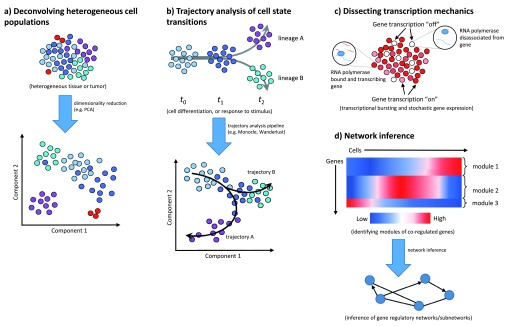
\includegraphics[width=\textwidth]{figures/biological_introduction/sc_purposes.jpg}
         \label{subfig:sc-applications}
         \caption[\textbf{Common applications of single-cell RNA sequencing}]{(a) Deconvolving heterogeneous cell populations. The single-cell resolution level can enhance the identification of rare cell species or subtypes. (b) \textit{Trajectory analysis} of cell state transitions, over the course of dynamic processes such as differentiation or signalling responses to an external stimulus. Recent computational advances, such as Monocle2 \autocite{qiu_etal17} can even reconstitute diverging and lineage-specific trajectories. (c) Dissecting the intricacy of transcription kinetics, inherently stochastic. (d) Network inference. Genes can be clustered by expression profiles to identify modules of co-regulated genes, further unravelled through studying the covariance matricial structure to infer gene regulatory networks. Reproduced from \autocite[Fig .1]{liu_trapnell16}.}
     \end{subfigure}
     \vfill
     \begin{subfigure}[p]{0.4\textwidth}
         \centering
         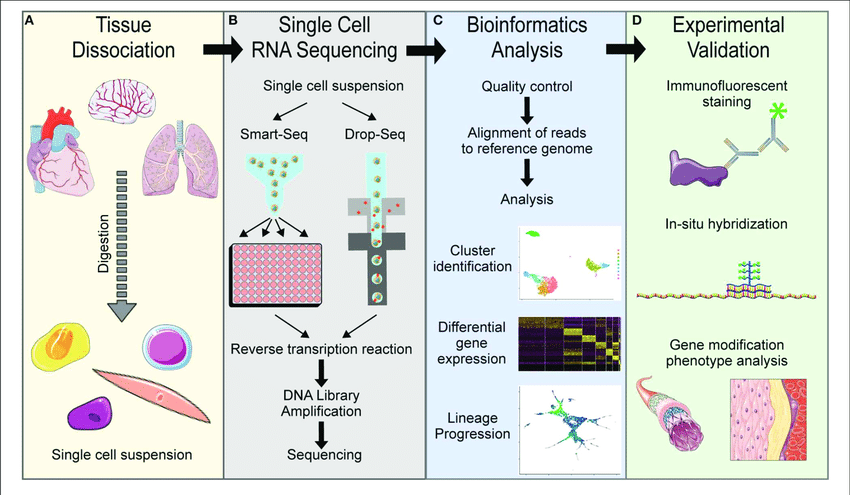
\includegraphics[width=\textwidth]{figures/biological_introduction/sc_pipeline.png}
         \label{subfig:sc-pipeline}
         \caption[\textbf{Overview of a standard single cell RNA sequencing pipeline}]{(A) Tissue dissociation at the cellular level (B) Single cell RNA sequencing of the single cell suspension. (C) Bioinformatics analysis of the library of reads sequenced (see \Cref{subfig:sc-nexflow} for an example pipeline). (D) Experimental validation. Reproduced from \autocite[Fig. 2]{chavkin_hirschi20}.}
     \end{subfigure}
     \hfill
     \begin{subfigure}[p]{0.58\textwidth}
         \centering
         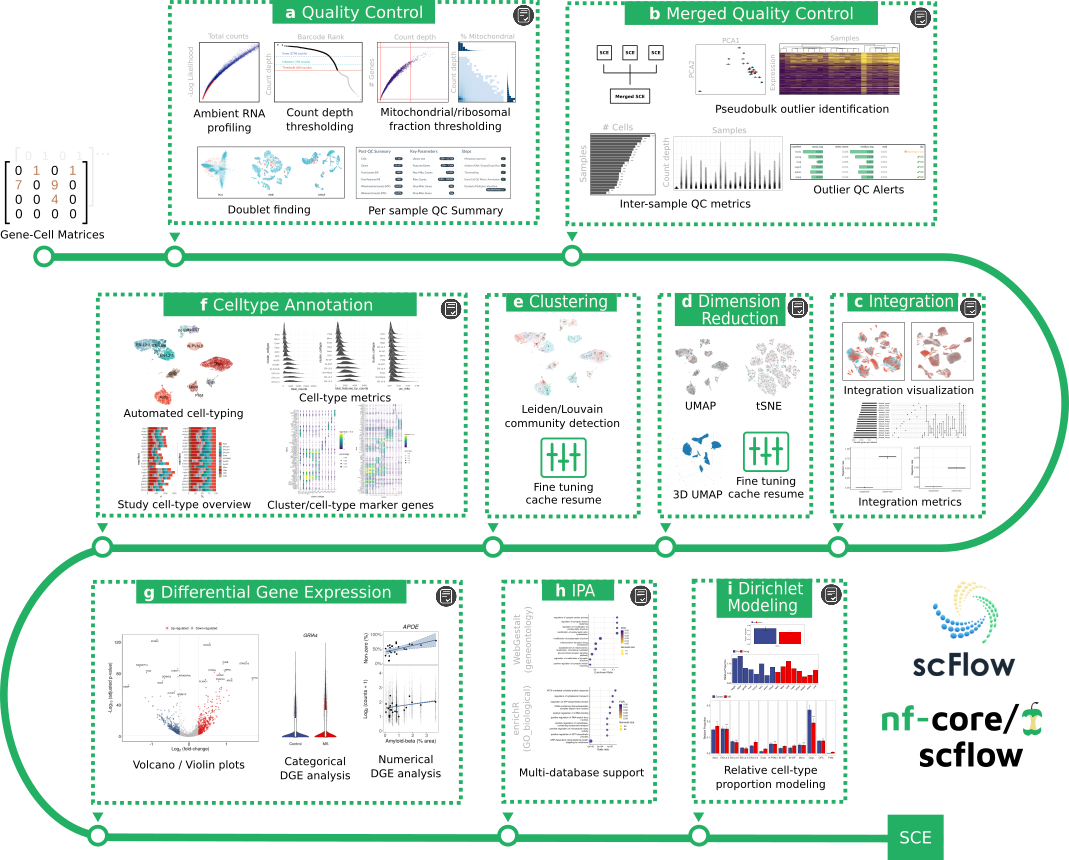
\includegraphics[width=\textwidth]{figures/biological_introduction/sc_computational_workflow.png}
         \label{subfig:sc-nextflow}
         \caption[\texttt{scflow}\textbf{: A Nextflow computational pipeline to analyse scRNA-Seq data}]{(a) Sample quality control including thresholding, doublet identification and removal of dead cells/ empty droplets. (b) Sample outlier identification. (c) and (d) Visualisation of high-dimensional datasets using non-linear dimensionality methods, such as UMAP \autocite{becht_etal19} or tSNE \autocite{maaten_hinton08}. (e) and (f) Louvain clustering \autocite{blondel_etal08} and automated cell-type annotation using marker gene sets. (g) Differential gene expression. (h) Pathway analysis, applying IPA \autocite{kramer_etal14}. (i) Address the inherently compositional nature of cell proportions (unit-simplex constraint) through Dirichlet modelling (see \Cref{sec:perspective-deconvolution} for details) and testing of cell-type composition changes. Reproduced from \autocite{khozoie_etal21}.}    
        \end{subfigure}
\end{figure}

\subsubsection{Spatial transcriptomics}
\label{subsec:st}


While \acrshort{scrna} enables to deconvolve cell populations within a tissue, it does not capture their spatial distribution, nor reveal in real time, \emph{in situ} cellular mechanisms. Indeed, the first step of the  \acrshort{scrna} protocol, namely the library preparation, is a destructive process \autocite{tang22}, which may induce unwanted expression, \enquote{ectopic} (expression not expected to occur in that tissue location), or resulting from the stress induced by the lysis process. This ultimately leads to a suboptimal characterisation and wrongly assignment of cell populations \autocite{vandenbrink_etal17}. 


Precisely, \acrshort{st} methods aim to characterise gene expression profiles while keeping the spatial tissue context. \acrshort{st} encompass two main techniques, each with its strengths and limitations (see also \Cref{subfig:spatial-transcriptomic}): 

\begin{itemize}
  \item \textbf{Image-based approach:} It comprises \emph{in situ} sequencing (ISS, \autocite{yokota_etal20}) and \emph{in situ} hybridisation (ISH, \autocite{vickovic_etal19}), both methods using probes to target specific genes. 
  ISS-based methods increase the amount of transcripts available for sequencing by rolling \emph{amplification} within the tissue after a step of reverse transcription. Each amplified transcript is unequivocally mapped back to its original material and localisation by a padlock probe which encodes an unique ID for each original transcript in each individual cell. Regarding ISH, target sequences are hybridised with a complementary fluorescent probe. 
  While both methods were originally limited in the number of distinguishable transcripts, relying on an unique fluorescent barcode for each transcript, recent developments involving multiplexing with sequential rounds of hybridisation (hence qualified HighPlex RNA imaging (HPRI, \autocite{he_etal22})) and imaging enabled an exponential  computational analysis: with $n$ distinct fluorescent colours and $k$ rounds of re-hybridisation and fluorescence to set apart $k^n$ distinct transcripts.
  
    Both techniques exhibit a strong bias and a lower coverage of the whole genome since they require a prior selection of target genes. Thus, they can not be used to track the apparition of unidentified isoforms or point mutations.  Finally, reads are generally noisier, especially due to the \emph{molecular crowding} phenomena, resulting in spatial overlap of fluorescence signals and restraining the number of fluorescent tags used to a few dozens. However, their single cell resolution (only limited by optical considerations, currently around $\sim \SI{100}{\micro \metre}$) and their better detection and depth per transcript make them better candidates to track temporal dynamics and their influence on the population layout. 
    
    \item \emph{in-situ} capture is a contemporary method that measures the transcriptome level for each of the individual spots of a finely-tuned lattice and tag it with an unique spatial \enquote{ID} barcode, with the spatial coordinates of the associated spot. Then, the sequencing step simultaneously reconstitutes the series of nucleotides composing the original mRNA fragment and map it back to its original spot, a technique consistently termed \emph{spatial barcoding} (see also \Cref{subfig:spatial-barcoding}). One of the current best performing methods, Visium, released by 10x Genomics, displays an increased resolution ($\SI{55}{\micro \metre}$ in diameter) and sensitivity ($\sim \num{10000}$ transcripts per spot) \autocite{nikhilrao_etal20}. 
    Although the sequencing throughput of NGS-based techniques employed in \acrshort{st} is orders of magnitude smaller compared to traditional \acrshort{RNA-Seq} technology, they similarly quantify in an agnostic manner the transcriptome expression, exhibit a higher coverage of the transcriptome compared to the Image-based approach and are cost-saving processes. 
    
    However, the design of the lattice of spots (either a microarray slide or a tangle of beads tethered in well structure, such as HDST \autocite{vickovic_etal19} or Slide-Seq \autocite{rodriques_etal19}), impacting the final \emph{resolution} capture (namely the distance between capture spots), is constrained by physical limitations. Accordingly, it is not rare that the mRNA captured at each spot represents a mixture of cells, rather than an individual entity. In addition, the standardised surface of capture, imposed by manufacturer norms and the computational burdensome of imaging development, may not be adjusted to the biological phenomena or the tissue studied.  
    To mitigate this issue, continuous enhancement of capturing techniques and miniaturisation tends to alleviate these physical and biological considerations, increasing by several factors the spatial resolution and the transcriptomic amplification:  Seq-Scope \autocite{cho_etal21} henceforth sequences at the subcellular resolution, while Pixel-Seq \autocite{fu_etal21} increases by $\sim 200$ folds the depth sequencing while claiming on average a resolution at the single cell size level ($\sim \SI{1}{\micro \metre}$).
    
\end{itemize}

Both techniques return a three-dimensional tensor of transcriptomic expressions, each gene being represented by a matrix of intensities representing its 2D (or even using computational assembling 3D) spatial expression pattern, resulting in the colourised Heatmap pictured in \Cref{subfig:spatial-barcoding}. 


The intricacy of \acrshort{st} is likely to reveal new biological insights, unavailable to standard transcriptomic methods, by adopting an hypothesis-free approach. In ~\autocite[Fig.~2]{rao_etal21}, direct applications from \acrshort{st} are reviewed, adopting a multi-layered view, from the local scale (the cell composition and gene composition of each spot) to the tissue level (detection of \enquote{spatial patterns} or \emph{hotspots}) \footnote{
By capturing in-place, and even in some cases, in-real time, the emph{co-localisation} distribution between hotspots of interacting cell types, \acrshort{st} can infer the intercellular communication patterns.  This approach can be employed, for instance, to strengthen or on the contrary, early discard putative biological interactions between a receptor and its ligand. Computational predictability of interactions arise from literature review, molecular screening, or \acrshort{scrna} correlation analysis (see \Cref{chap:covid19} for a review of physical and computational approaches to predict drug-target interactions notably). Even with robust evidence of physical interaction, if two distinct cell subpopulations are spatially distant and cannot effectively communicate, the possibility of intercellular exchanges is unlikely: indeed, as quantified in \autocite{armingol_etal21}, a significant portion of cellular signalling occurs within the neighbourhood of the releasing cell, operating at the juxtacrine and paracrine levels within a range of \qtyrange{0}{100}{\micro\meter}. This heuristic technique of checking conjectured intercellular communications through co-localisation analysis is visually described in \autocite[Figure 5]{longo_etal21}, and is notably used by SpaOTsc \autocite{cang_nie20}.}. 
Besides, since \acrshort{st} tend to be less destructive compared to other exploratory approaches, preventing structural damage or further cell death, they are intensively used to survey temporal dysregulation patterns of complex, intertwined systems, with applications ranging from neurodegenerative disorders (Alzheimer’s disease \autocite{chen_etal20}, AML \autocite{warnat-herresthal_etal20}) to immuno-inflammatory affections (influenza, \autocite{curras-alonso_etal21}, sepsis, \autocite{janosevic_etal21}). 

\begin{figure}
     \centering
     \begin{subfigure}[p]{0.45\textwidth}
         \centering
         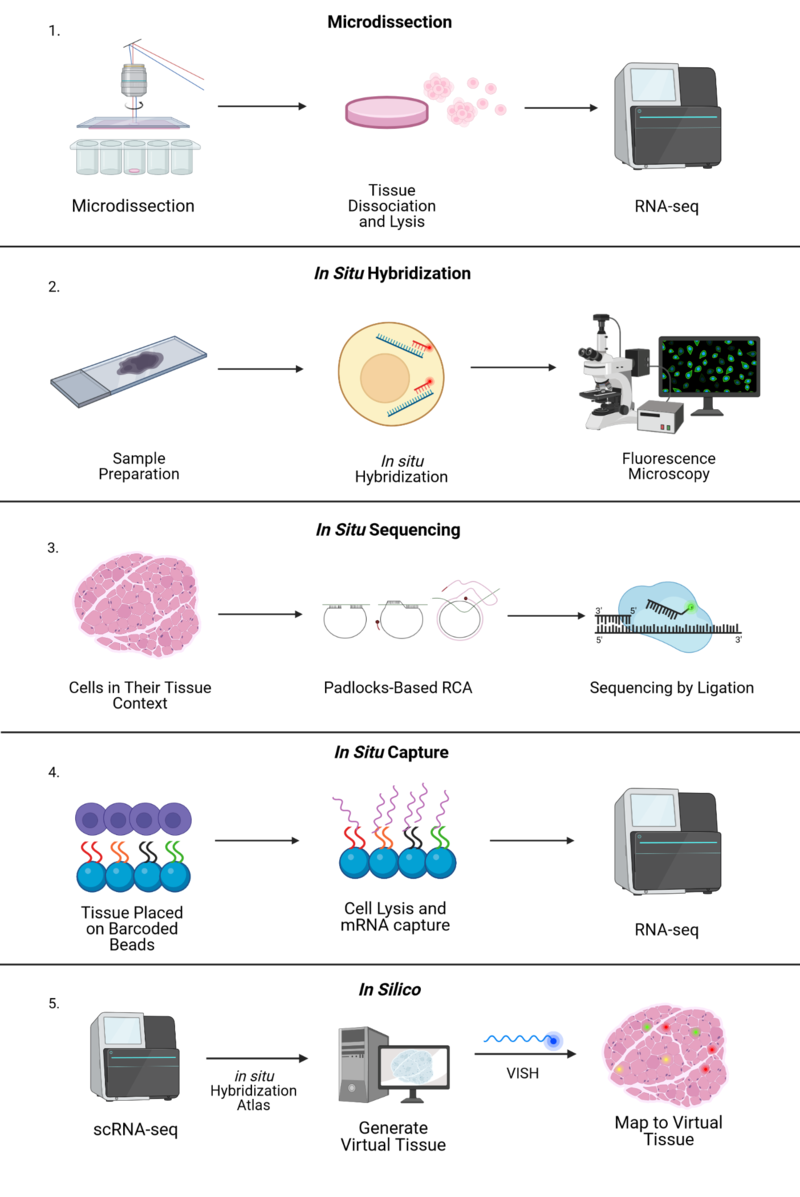
\includegraphics[width=\textwidth]{figures/biological_introduction/Spatial_Transcriptomics_Overview.png}
         \label{subfig:spatial-transcriptomic}
         \caption[\textbf{Overview of Spatial Transcriptomics Methods}]{(1) Microdissection method. (2) \textit{in-situ} Hybridisation method. (3) \textit{in-situ} Sequencing method. (4) \textit{in-situ} Capture method, alternatively named spatial barcoding. (5) \textit{in-silico} method. Reproduced from \autocite[Fig .1]{slifertheryedragon23}, using the BioRender software \autocite{biorender}.}
     \end{subfigure}
     \hfill
     \begin{subfigure}[p]{0.45\textwidth}
         \centering
         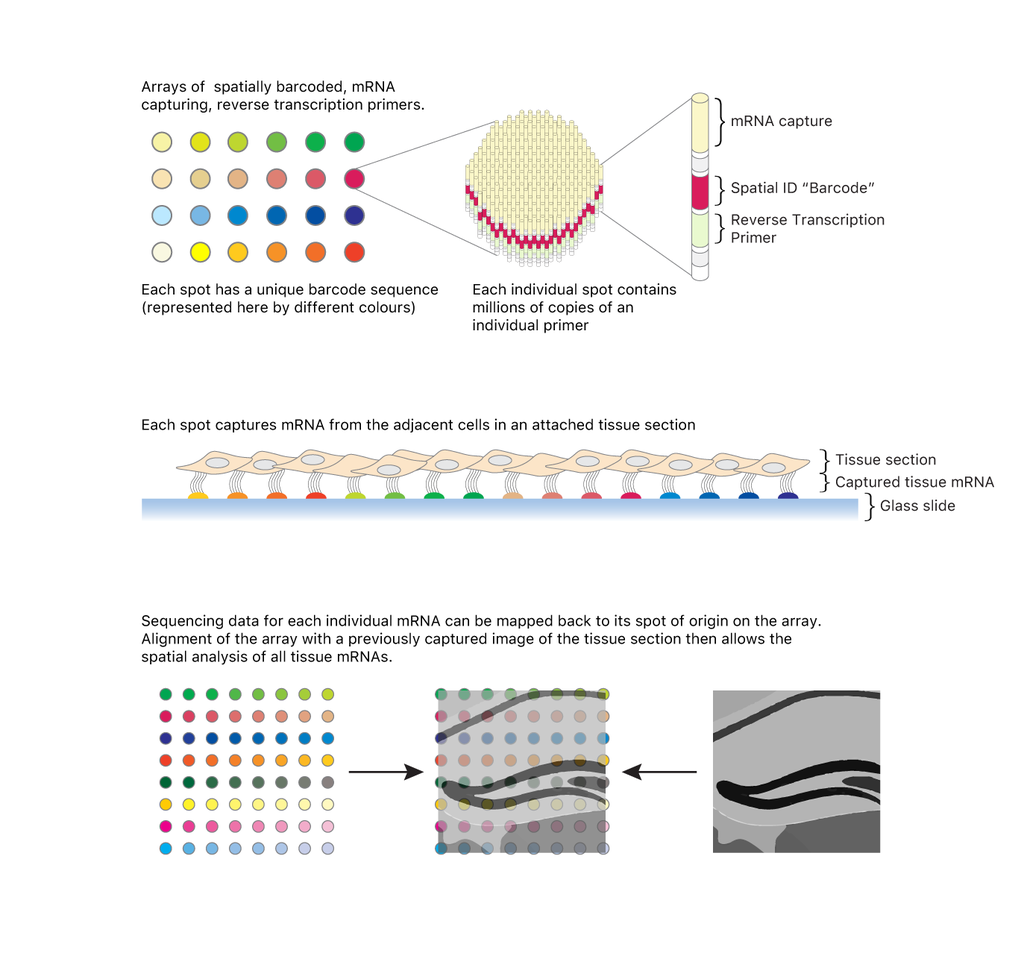
\includegraphics[width=\textwidth]{figures/biological_introduction/Spatial_transcriptomics_detail.png}
         \label{subfig:spatial-barcoding}
         \caption[\textbf{Zoom on the \textit{spatial barcoding} technique}]{Reproduced from \autocite[Fig. 3]{chell23}.}
     \end{subfigure}
     \vfill
     \begin{subfigure}[p]{0.95\textwidth}
         \centering
         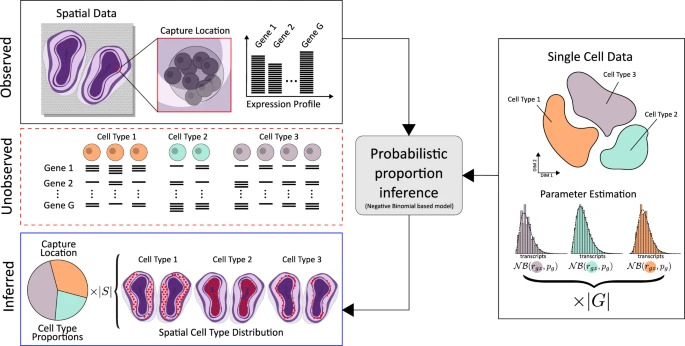
\includegraphics[width=\textwidth]{figures/biological_introduction/sc_deconvolution.jpg}
         \label{subfig:sc-deconvolution}
         \caption[\texttt{stereoscope}\textbf{: A single cell, spatial deconvolution algorithm}]{A deconvolution algorithm is used to model and infer the mixture composition of cell populations at a specific capture site, using annotated single-cell data. Interestingly, the method does not rely on marker genes or gene set enrichment to quantify the cellular composition.  Precisely, the probabilistic model employs a convolution of negative binomial distributions to yield a comprehensive map of the spatial distribution of cell types throughout the entire tissue. Reproduced from \autocite{khozoie_etal21}.}         
         
     \end{subfigure}
\end{figure}

The next bioinformatic milestone in the area is the reconstruction of a real multi-layered model, the only means of unravelling how emerging properties arise from the spatial arrangement and individual cell-cell interactions: promising approaches integrating this aspect are briefly reviewed in my general author's opinion in \Cref{chap:general-perspectives}. 

\subsubsection{The best of both worlds: towards a holistic biomolecular approach}
\label{subsec:sc-and-st}

Nonetheless, the restricted transcriptome \emph{coverage} and \emph{depth} associated with \acrshort{scrna}-\acrshort{st}-based approaches impede their capacity for in-depth exploration, suggesting to bridge both worlds, coupling the versatility of \acrshort{st} investigations with the precision and accuracy offered by \acrshort{RNA-Seq} technologies. An integrative approach is more amenable to unravel the mechanistic processes underlying intricate biological processes, ranging from capturing the temporal dynamics of tissue development through \gls{lineage tracing} \autocite{zhang_etal20} or RNAVelocity \autocite{lamanno_etal18} (\autocite{asp_etal19} applied \acrshort{st} on cardiomyocyte populations at the embryonic stage) to understanding the temporal dynamic involved in the pathogenesis progression (\autocite{maniatis_etal19} identifies a set of 31 co-expression modules temporally correlated with the evolution of amyotrophic lateral sclerosis, coupling spatial barcoding with \acrshort{scrna}). 


There are two primary approaches for integrating \acrshort{scrna} in spatial data: \emph{cellular deconvolution} (see \Cref{sec:perspective-deconvolution} for details) and \emph{mapping}. 

Both methods follow the same workflow subdivided into four stages, often referred to as the four A's (\autocite[Fig. 4]{longo_etal21}):
\begin{itemize}
    \item \textbf{Adopt} From literature, a subset of the tissues or the populations of interest, with intricate spatial patterns, is selected for further analysis. 
    \item \textbf{Assay} Survey the same tissue (to keep the same phenotypical conditions and limit technical variability) with scRNA-sequencing (its higher coverage and unbiased nature makes it a promising candidate for the selection of candidate genes) and spatial barcoding to locate their prevailing location within the tissue. Then, track the spatial and temporal dynamics of this subset of genes with HPRI imaging (recall that this method requires to know in advance the sequence of the genes).
    \item \textbf{Assemble} Using deconvolution and mapping algorithms, generate maps that assigns each coordinate to one cell type. Matching histology images may reveal informative landmarks and help denoising complex areas, such as the tumour leading edge, transition region between cancer and normal tissue. 
    \item \textbf{Analyse} The high-dimensionality of \acrshort{st} datasets was use to corroborate ligand-receptor interactions involved in cellular signalling, or to survey evolving dynamics occurring in a disease progressing condition.
\end{itemize}

\textit{Mapping}, generally employed for high-plex RNA imaging assays, consists first to assign each spatially detected cell to its corresponding (scRNA-seq) profile and secondarily, infer a pattern predicting the location of each scRNA-seq cell based on its transcriptome. Mapping reveals notably useful to determine the general layout of cell populations within a tissue and to identify hotspots or \enquote{niches} (specific and localised microenvironments in which stem cells prevail over fully differentiated cell subtypes). A benchmark of fourteen algorithms that implement mapping through cluster-based approach \autocite{tran_etal20} states that the three best performing were LIGER \autocite{welch_etal19}, Seurat Integration \autocite{stuart_etal19} and Harmony \autocite{korsunsky_etal19}). All three algorithms ultimately retrieve cell types by clustering joined \Gls{st} and scRNA-seq data, which was first projected to a lower-dimensional space. 


Furthermore, instead of surveying only one omic, capturing the simultaneous spatial and temporal evolution of heterogeneous biological data is likely to even increase the exploratory avenues offered by these promising technologies. Hence, \acrshort{scrna} is paired with orthogonal omic information, respectively with epigenomics \autocite{smallwood_etal14}, genomics \autocite{dey_etal15} or proteomics \autocite{amir_etal13}). Another promising avenue aims at integrating within high-resolution tissue images histopathology annotations, such as the cell shape or size. Traditionally, the methods took profit from canonical in-situ hybridisation technics (FISSEQ \autocite{lee_etal14}, TIVA \autocite{lovatt_etal14}) or RNA tomography (Tomo-Seq, \autocite{holler_junker19}).  Another recent alternative is the \emph{stochastic profiling} approach: instead of prospecting at the single cell level and hereby, dealing with small amounts of RNA, this method aggregates the expression of randomly chosen and heterogeneous small pools of cells (around a dozen), increasing the amount of mRNA produced. Then, deconvolution algorithms (\autocite{narayanan_etal16} and  \autocite{andersson_etal20}), are used to computationally dissect the pool of $k$ cells at the individual cell level. To that purpose, \autocite{andersson_etal20} developed a probabilistic framework, named \texttt{stereoscope}, that combines single-cell and $k$-cell data to infer robust and accurate evaluation of the intracellular heterogeneity. Precisely, the distribution of the transcripts are modelled through negative binomial distributions, which are further employed to study the heterogeneous activation patterns from key regulatory genes, as depicted in \Cref{subfig:sc-deconvolution}. 


We refer the interested reader to \autocite{longo_etal21} and \autocite{williams_etal22} for a comprehensive review of spatial transcriptomic and \acrshort{scrna} technologies, with their respective advantages, limitations and computational resources to analyse them.



\subsection{Miscellaneous applications of ngs technologies}
\label{subsec:miscelleanous-innovative-rna-seq}

The versatility of \acrshort{ngs} platforms enable a wide variety of genomic, transcriptomic or epigenomic applications, beyond the mere quantification of known transcripts. In these applications, while the sequencing process is shared across applications, the RNA or DNA library preparation and the bioinformatic algorithms to map and analyse the reads have a strong impact on the accuracy of the downstream analysis performed. 
A brief overview of other applications is described hereafter:

\begin{enumerate}[label=(\roman*)]

\item \textbf{Genomics sequencing:} Three applications benefit from the high-throughput sequencing process of \acrshort{ngs}: WGS (whole genome sequencing), WES (whole exome sequencing) and \emph{de novo} sequencing. Genome-wide association studies(GWAS) are a common approach for identifying disease association patterns across the whole genome: while relying previously on a final set of pre-defined markers interrogated by microarray-based methods, the most comprehensive method of interrogating the 3.2 billion bases of the whole human genome has only emerged with the more scalable and flexible \acrshort{ngs} technology.  In order to decrease the costs, it is also possible to focus only on the set of protein-coding sequences (the exome), since they  gather most of the known disease-causing variants. 

\item \textbf{Transcriptomics} In addition to total mRNA sequencing already discussed comprehensively in \Cref{subsec:RNASeq}, it is also possible to target only transcripts or a specific region of interest to both save costs and get a comprehensive insight on the intricacy of the regulation mechanisms involved, ranging from alternative splicing with isoforms to mRNA mutations or modified enhancer sequences. Notably, targeted resequencing projects has typically a coverage of $500-1000 \times$ against an average of $30\times$ for traditional WGS projects \autocite{li_etal15} \autocite{johansson_etal11}. Such a strategy increases the possibility to detect rare variants, notably somatic mutations in highly-heterogeneous samples (e.g., in the Tumoral MicroEnvironment, with a variety of tumoral clone populations mingled with germline or cells displaying a healthy phenotype).
Finally, it is possible to select upstream microRNAs (short, non-translated nucleotide sequences) that were shown to play a role in the regulation of gene expression (\Cref{subsec:reg-transcript}, \autocite{catalanotto_etal16}, \autocite{moreno-moya_etal14}).

\item \textbf{Epigenomics} Epigenetics aims at understanding the mechanisms underlying the regulation of the transcriptome, deprived from mutations on DNA sequences' causes. This notably includes DNA methylation, smallRNA mediated regulation and PPI interactions with the genome \Cref{sec:gene-regulation}.

\emph{Methylation sequencing} focuses generally on highly regulated regions, such as promoters or heterochromatin, generally enriched in GC sequences, and require specific \acrshort{ngs} technologies able to dive down to the nucleotide level \autocite{zmarzly_etal16}, \autocite{coleman-derr_zilberman12} and \autocite{han_etal07}. The two major methylation methods are Whole-Genome Bisulfite Sequencing(WGBS, \autocite{zhou_etal19a}) and Reduced Representation Bisulfite Sequencing (RRBS, \autocite{sang21} and \autocite{wan_bell20}). 

\emph{protein–DNA interactions} can be precisely surveyed, combining the high-throughput sequencing of \acrshort{ngs} with Chromatin Immuno-Precipitation Sequencing (ChIP-Seq) \autocite{small_etal21}. These methods are used to identify the binding sites for a given protein at the scope of the whole genome. 

\emph{Ribosome profiling} focuses on mRNA strands that migrate to the ribosome complexes, in which they are translated into proteins. Hence, this technique provides a more faithful insight at the protein level compared to classical RNA sequencing (RNA-Seq) \autocite{blevins_etal19}. This information enables an indirect quantification (straightforward to get, compared to direct quantification measures) of the proteome (set of proteins currently translated/produced in the cell), hereby providing an insight on post-transcriptional regulation mechanisms \Cref{subsec:post-transla}, \autocite{kiniry_etal20}, \autocite{yadav_etal21}.   

While some regulation processes occur in localised regions of the genome, other processes modify globally the rate of transcription by acting on the \emph{tridimensional spatial configuration} at the genome scale \Cref{subsec:reg-transcript}. \emph{Chromatin remodelling} is one of the key mechanism involved and is estimated through the combination of \acrshort{ngs} technologies with the ATAC (Assay for Transposase-Accessible Chromatin) technology \autocite{ahmed_ucar17} \autocite{sahu_etal21}.
\end{enumerate}

\section{A glance at the world of immunology}
\label{sec:immunology}
\todo[fancyline]{thèse d'étienne, présentation bio Servier \enquote{Immunology at a glance}, chapter 43 about the immune system}

\paragraph{Overview: the  immune system, the keeper of our body} 
\
The immune system is an intertwined network of cells, organs and molecules that work together to protect the body against infectious agents that may reveal harmful for organism. Such threats are collectively named \emph{pathogens}, ranging from viruses to bacteria and fungi. Its primary role is to early recognise these intruders, in order to eliminate them quickly. The main concept here is to rapidly discriminate foreign molecules as well as self compartments such as tumoral cells that may have a pathogenic effect, from innocuous particles or self sections, for whom no immune reaction is expected. An adjusted \emph{molecular recognition} is a key feature of the immune system, as perturbations of its mechanism is at the origin of the vast majority of immune disorders. 

The immune system is traditionally divided into two interacting schemes: the \emph{innate immune system} and the \emph{adaptive immune system}. 
Ultimately, the immune system plays a crucial role in keeping the homeostasis of the human body, by defending against a wide range of infectious diseases or inner dysregulations. 

\subsection{The innate system}
\label{subsec:innate-system}
The innate immune system is the first line of defence and provides immediate, \emph{non-specific} protection against invading pathogens.  This includes:
\begin{itemize}
    \item \textbf{Barrier defences} Physical barriers, such as the skin and mucous membranes, are the first line of defence, preventing pathogens from accessing the inner environment. However, entire sealing is impossible, since the human organism must interact with its environment, through gas exchange and nutrition to maintain homeostasis and perform vital biochemical functions. Thus, these protections are generally completed with chemical secretions trapping pathogens, specialised organelles such as lysosomes and reservoir of innate cells poised to fend off potential invasion. Finally, the mucous membranes (from mucus, a viscous fluid aimed at trapping viral particles) of the \gls{epithelial} tissues, such as the digestive or airway tract, provide additional barriers to infection. In parallel with the production of mucus, saliva and other enzymes secreted provide a washing action that inhibits colonisation by fungi and bacteria, destroy their cell walls and contribute to the acidity of the medium, killing most of susceptible bacteria.  
    
    \item \textbf{Immune cells} Cellular defence mechanisms rapidly identify proteins that are commonly shared among pathogens by utilizing specialized receptors on their surfaces. Among these, the Toll-like receptors (TLRs) family, for which the Nobel Prize in Physiology was awarded in 2011, holds a prominent place: this class of proteins is remarkably widespread in the animal kingdom, capable of recognising a diverse panel of micro-organisms \autocite{akira_takeda04}. For example, the TLR3 complex binds to double-stranded RNA, a common nuclic organisation in viruses \autocite{matsumoto_seya08} while the TLR4 and TLR5 respectively target the lipopolysaccharide found on the surface of many bacteria \autocite{takeuchi_etal99} and flagellin \autocite{gewirtz_etal01}, the main protein of bacterial flagella. 

    Then, the elimination process differs along with the nature of the cell. \emph{Macrophages} (\enquote{big eaters}) and \emph{neutrophiles} wipe out pathogens that breach the natural physical barriers by \emph{phagocytosis}. Phagocytosis, originating from the Greek term \enquote{cell eater} is the intricate process through which phagocytes internalise and digest foreign intruders and dead cells. After a first recognition stage, the phagocyte encapsulates the intruder in the phagosome, then fuses within its cytoplasm with the lysosome organelle, whose enzymescut into several pieces the foreign molecules. Generally, influx of neutrophils precedes the arrival of monocytes that rapidly differentiate into macrophages within tissues. 
    
    \emph{Natural killer cells} can induce the death of virus-infected cells \footnote{The term \enquote{natural} stems from their direct action, without prior exposure or activation, while the neutralisation mechanism is akin to the TCD8 cell type. Additionally, they are strongly related to lymphocytes involved in adaptive immune response (\ref{subsec:adaptive-system}, making part of a third component}. NK cells proceed by first detecting abnormal surface-receptors proteins, such as stress signals or tumour antigens, and then by releasing toxic molecules that trigger \emph{apoptosis}, a programmed death of the stricken cell. 
    
    More specialised cells involve \emph{dentritic cells}, whose main function is to coordinate the innate and the adaptive response \ref{subsec:collab-innate-adaptive}, \emph{mast cells} contribute to the inflammatory response but are also involved in aberrant reactions such as allergies, along with \emph{eosinophils} and \emph{basophils}, whose original function was the protection against multicellular parasites, such as worms, that usually require an even stronger reaction. 
    
    \item \textbf{Signalling and antimicrobial proteins} While some peptides directly target and induce destruction of pathogens, such as the \emph{complement system}, others dedicate as regulators and coordinators of the immune response. The complement system is a set of of 30 identified proteins in blood plasma that interact with each other in a highly coordinated and sequential manner. This cascade of biochemical reactions leads to the formation of protein complexes that trigger the \emph{lysis} of invading cells (destruction through bursting of the membrane), the opsonisation (marking for destruction) and the recruitment of immune cells to the site of infection. In addition to its role in fighting infections, the complement system also plays a role in other biological processes, such as tissue repair and development.
    
    Interferons interfere with  cells hosting virus, through mechanisms depending on their belonging class: $\alpha$, $\beta$ and $\gamma$. Interferons are released by virus-infected cells and by binding to neighbouring immune cells, they inhibit viral replication or promote the phagocytic ability of macrophages.

    Cytokines can be released by macrophages, dendritic cells, and natural killer cells. While some of them, such as interleukin-1 (IL-1) and tumour necrosis factor alpha (TNF-alpha), promote inflammation by recruiting neutrophils to the site of infection, others, on the contrary, such as interleukin-10 (IL-10) and transforming growth factor beta (TGF-beta) resolve inflammation and promote tissue repair.  
    
    \item The \emph{inflammatory response} (from Latin \emph{inflammare}, \enquote{set on fire}) is the set of events that modify the microenvironment, triggered by an intertwined cellular signalling released upon infection. The first stage often involves mast cells secreting cytokines, such as \emph{histamine}, that promote growth, migration, and activation of endothelial cells, thus contributing to \emph{vasodilation} \autocite{ribatti_etal20}. The dilatation of blood vessels causes the well-known, localised inflammatory response, characterised by the increase of the skin temperature, redness, and enhanced blood flow. Besides, the released cytokines promote the migration of immune cells towards the inflamed region through a process called \emph{chemoattraction} (movement of a cell following the chemical gradient of a signalling molecule). Then, cycles of signalling and response keep on sustaining the inflammation process, with the deployment of the complement system and the continuous recruitment of additional immune cells \autocite{mollaei_etal20}. 

\end{itemize}

For a faster response, it is worth noting that the two main components of the inflammatory response, namely the macrophages and neutrophiles, circulate throughout the body through the lymph system, whereas others reside permanently in organs and tissues, increasing the likelihood to encounter pathogens and a prompt immune response. However, this first line of defence may reveal insufficient to fend off particularly harsh pathogens strengthened by millions of years of co-evolution. Indeed, some pathogens evolve specifically to overbalance the immune defences (a set of mechanisms referred to as \emph{immune escape}), with some bacteria have an outer capsule that prevents recognition, while others are resistant to breakdown within lysosomes. 


\subsection{The adaptive system}
\label{subsec:adaptive-system}
The adaptive immune system, on the other hand, provides a targeted response to pathogens that have already overwhelmed the innate system, through receptors specific to the intruders. Adaptive immunity relies on two types of lymphocytes: B cells and T cells \footnote{Like all blood cells, lymphocytes originate from stem cells in the bone marrow, but while T cells migrate to the thymus, B cells undergo their maturation stage in the bone marrow. Generally, \Gls{hematopoiesis} is the biological process involved in renewing all the cell populations circulating in the blood, while the corresponding scientific field focuses on resolving their lineage relationships.}. 

All receptor proteins on a single B or T cell share the same antigen receptor and recognise the same \emph{antigen}, any foreign molecule detected as non-self and able to elicit recognition (typically, around \num{100000} are present on their surface). To recognise any potential antigen, millions of distinct lymphocytes coexist in the body, each with its own recognition pattern, able to either bind to a protruding antigen surface or circulating agent, such as microbial toxins. 


The adaptive immune response decomposes into four stages:
\begin{enumerate}[label=(\alph*)]
    \item \textbf{cell diversity} This step enables the creation of a large repertoire of unique lymphocytes, which in turn allows for recognising a large pool of antigens, including theoretically even those never encountered \footnote{Studies show that one million of different B cell antigen receptors and 10 million different T cell antigen receptors coexist in the human organism}. Random \emph{alternative splicing} and \emph{gene recombination} are the fundamental somatic processes that facilitate the production of a comprehensive pool of unique sequence arrangements that compose the variable sections of antibodies. This mechanism is commonly known as \enquote{V(D)J recombination} \autocite{bassing_etal02} and is accomplished through a restricted set of genes  \footnote{The individual pieces composing the light chain of the antibodies can be combined in 200 different ways, and even more for the heavy chain, resulting in \num{3.5e6} possible combinations within the B cell repertoire \autocite{guo12}}. Once the original stem cell produces its own rearrangement of the antigen receptors, they remain permanent and are passed on to the daughter cells.
    
    \item \textbf{Self-tolerance} This step aims at eliminating self-reactive lymphocytes, namely those that recognise own molecules as non self, and thus could trigger improper immune reaction against the body's own molecules and cells. These self-reactive lymphocytes are either destroyed through apoptosis, or rendered non functional. 

    \item \textbf{Clonal selection and Cell Proliferation} The activation of the unique set of B or T cells requires the binding between the epitope of an antigen and an antigen receptor, with the match generally occurring in the lymph nodes \autocite[Figure 6, Chapter 43]{campbell_etal20}. But without clonal amplification, no effective adaptive response would be possible. 
    
    Once activated through binding to an antigen, lymphocytes proliferate into a clonal population, whose cells are all identical to the ancestor lymphocyte and bears the same antigen receptors. Then,  they become \emph{effector cells} and mediate a strong and personalised immune response through the action of (1) T CD4 or Th Helper that coordinate the adaptive response, through notably clonal amplification of effective lymphocytes, (2) T CD8 that kill cells infected
by viruses (\emph{host cells}) and (3) activated B cells, the \emph{plasma cells}, that produce soluble proteins called antibodies that circulate freely in the body fluids. The whole process is termed \emph{clonal selection} as only the lymphocytes specific for a particular epitopemultiply. 

Specifically, helper T cells only recognise antigens that are displayed by the class II MHC on the surface of antigen-presenting cells (APC), generally dendritic cells (DC), but it can also be macrophages or B cells. The specificity of the APC-Th Helper connection hinges on the CD4 protein that guarantees a strengthened joint and extensive information exchange between the lymphocyte and the APC. Once activated, TCD 4 secrete cytokines that promote the generation of a clonal population  and trigger two distinct immune responses that depend on the nature of the vector. The several missions and the crucial role of helper T cell as conductor of the adaptive response is summed up in \autocite[Figure 18, Chapter 43]{campbell_etal20}.

The \emph{humoral immune response} involves the release of antibodies by plasma cells, that in turn promote bacteria elimination by facilitating phagocytosis (act as markers of foreign cells) and promoting the complement response. The released antibodies do not directly kill pathogens, but by targeting circulating toxins or epitopes cradled by the class I MHC of infected cells, prevent viral infection or bacterial activity through \emph{\gls{neutralisation}} or \emph{opsonisation} mechanisms. 

The activation of B cells requires a two-factor authentication process: the first contact with a circulating antigen antigen in lymph nodes turns a virgin B cell into a mature B cell and starts clonal amplification. In the mean time, the activated lymphocyte engulfs some foreign molecules by endocytosis and displays them through its MHC class II molecules. Ultimately, it is only when the B cell meets an helper T cell that was activated in parallel by a macrophage or a dentritic cell that it can turn into an efficient Plasma Cell, a true antibody-secreting factory. This two-step activation is clearly described in \autocite[Figure 19, Chapter 43]{campbell_etal20} and in \autocite[Figures 1 and 2, Chapter 21]{dettmer21}. 

In the \emph{cell-mediated immune response}, another subset of T cells, the TCD 8, proliferate and differentiate into cytotoxic T cells. Initiation of the cell-mediated response first requires activation signals from Th Helper, while the identification of the cells to eliminate relies on the detection of an antigen fragment displayed by the class I MHC of infected cells. In a process similar to NK cells \ref{subsec:innate-system}, destruction of host cells involves the release of perforines that puncture the membrane structure (generate \enquote{pores}), leading to cell lysis, and granzymes that cleave essential proteins, leading to cell apoptosis. Cytotoxic T cells are also equipped with an accessory protein, the CD8 marker, that guaranties strong binding all along the destructive process \autocite[Figure 22, Chapter 43]{campbell_etal20}. Even though not directly targeting virus, depriving the pathogens from potential hosts reduces practically the magnitude and the propagation of the infection. 



\item \textbf{Immunological Memory} 
Finally, the immunological memory is responsible for the long-term protection elicited by a prior infection. This protective mechanism differs from the \emph{primary immune response} by a faster and prolonged response (peak intensity within two days against 10 days), with a greater magnitude (the concentration of antibodies or killer T cells increases by two or three folds). 

This heightened secondary response to the same antigen relies on a subset of the effector lymphocytes, called \emph{memory cells}, that were first activated in reaction to an initial exposure of an antigen. While the vast majority of lymphocytes are short-lived and are eliminated once the infection is overcome (notably by an other category of specialised T cells, depicted as \emph{regulatory}), the longer life duration places memory lymphocytes at the forefront to rapidly initiate clonal amplification of thousands of highly-specialised effector cells, in case of second exposure. 

This mechanism is directly leveraged for \emph{immunisation}, namely the artificial introduction of antigens into the body to generate a pool of memory cells. It is also referred to as \emph{vaccination} (from the Latin \enquote{vacca}, \emph{cow}), since the first documented use of the immunisation principle dates back to late 1700's, when Jenner observed that peasants contract the relatively innocuous cowpox disease, they were protected from the damaging outbreaks of smallpox. Nowadays, vaccines are made from killed or weakened pathogens (first generation), inactivated bacterial toxins (second generation, with careful selection of epitopes) or
even genes encoding microbial proteins (third generation, for instance the \enquote{Messenger RNA vaccines} developed by Pfizer or Moderna against the Covid19), all eliciting a first immune response. Vaccination programs enable to dramatically reduce the infant mortality caused by devastating diseases, whose vectors were particularly obnoxious due to their high pathogenocity combined with escape immunity mechanisms. Notably, the smallpox was eradicated in 1980, while polio and measles cases decreased by several folds.

\end{enumerate}


\subsection{Exchange of goodwill between the two immune systems}
\label{subsec:collab-innate-adaptive}

Contrary to the standard approach which opposes the innate system, shared by all animals, to the seemingly more efficient adaptive system, only developed among jawed vertebrates, we show in this point that it is the constant interplay between lymphocytes and other innate cells that together provides this efficient, coordinated and constantly remodelled protection against a variety of pathogens.

The cooperation between innate and adaptive system generates a positive feedback loop whose main stages are reported on \Cref{fig:innate-adaptive-cooperation}, emphasising how much these two systems are closely intertwined:

\begin{figure}
    \centering
    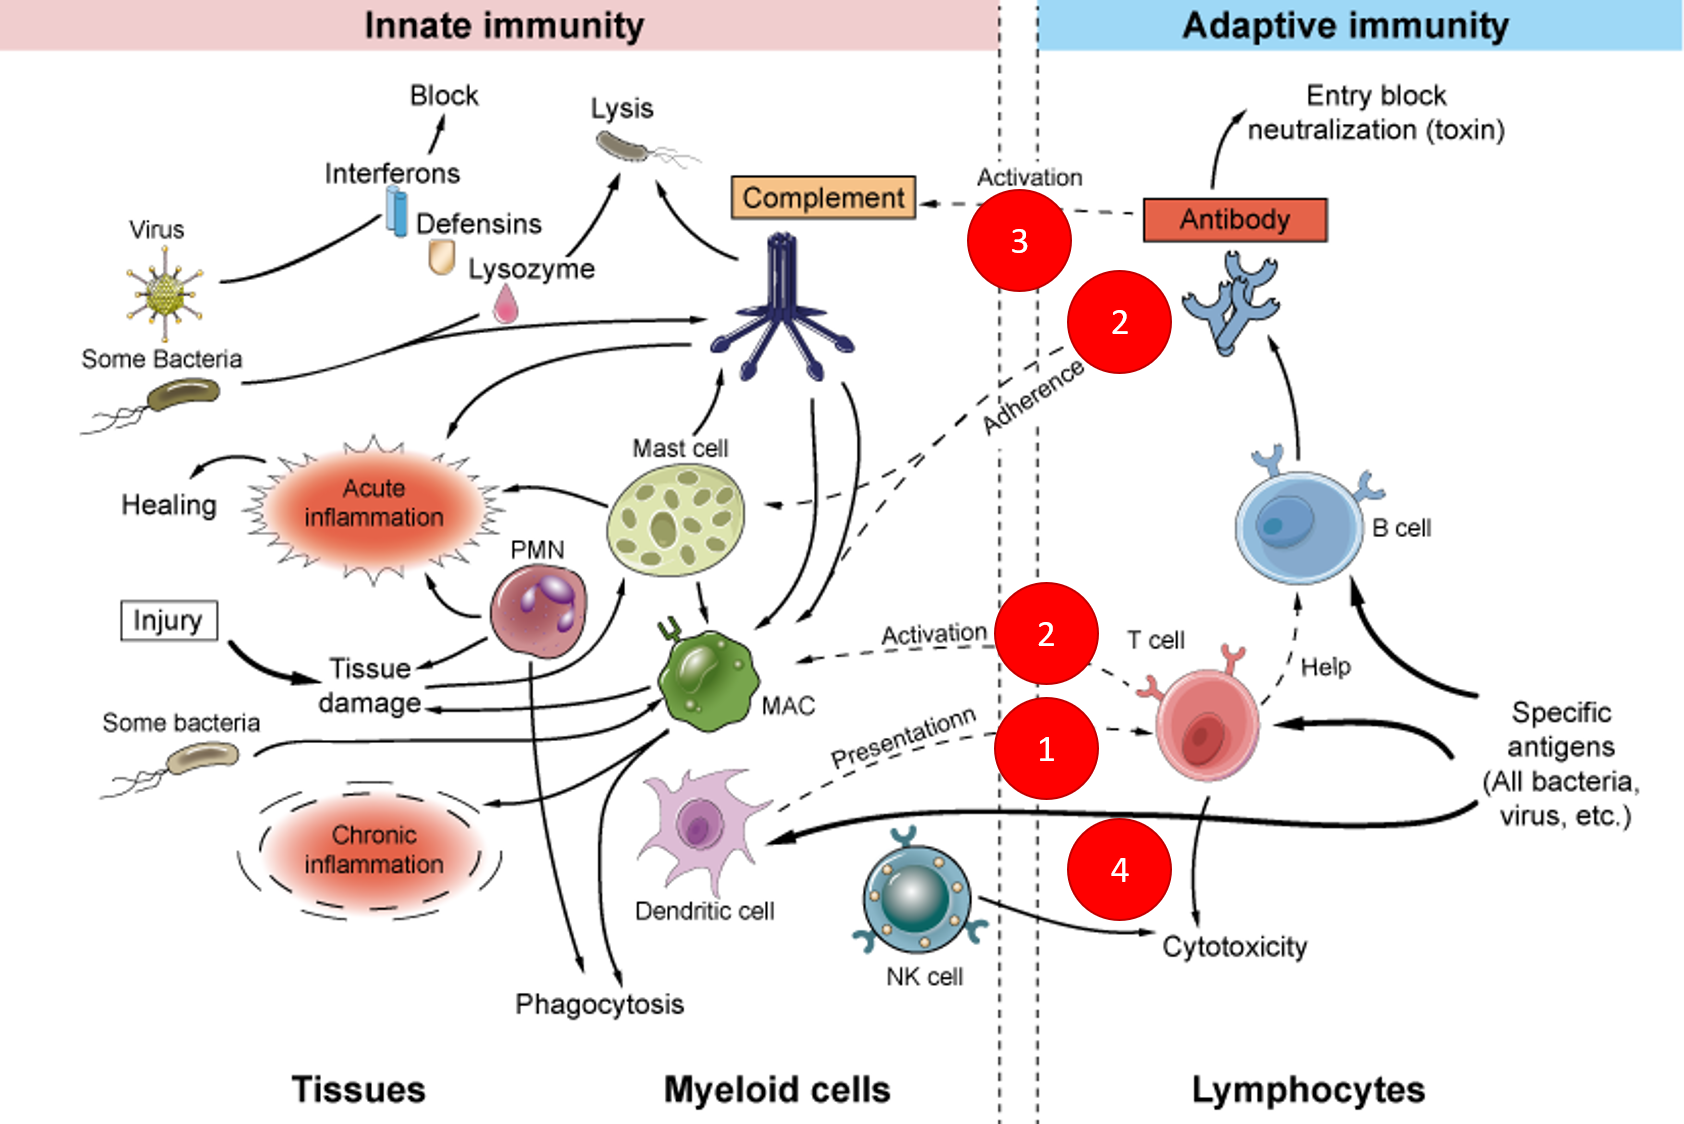
\includegraphics[scale=0.3]{figures/innate-adaptive-cooperation.png}
    \caption[Cooperation mechanisms between the innate and the adaptive immunity]{
    This iconography shows the inner mechanisms intervening in the innate (left) and adaptive (right) response, each able to trigger a cellular (lower half) or humoral reaction (upper half). Reproduced from \autocite[Fig .1]{cdcreativediagnostics20}.}
        \label{fig:innate-adaptive-cooperation}
\end{figure}
    
     However, adaptive mechanisms, although more recent in the evolution, need multiple interactions with the older innate one, reviewed in arbitrary chronological order below:
    \begin{itemize}
        \item A local inflammatory response generally produces \emph{pus}, a mixture of white blood cells, dead pathogens, and debris from damaged tissue, that is flushed away through the lymphatic system towards the lymph nodes, in which permanent macrophages can engulf recognise and display fragment antigens \autocite[Figure 12, Chapter 43]{campbell_etal20}. In the mean time, dendritic cells migrate to the lymph nodes after interacting with pathogens. 
        In both cases, the \emph{phagocytosis} pathway enables to trap antigens, cradled in the MHC II complex, by cleaving the foreign particle into smaller peptides. Finally, the interaction of the MHC with its antigen fragment and the TCR receptor of a TCD4 cell \autocite[Figures 12 and 13, Chapter 43]{campbell_etal20}, triggers an adaptive immune response, through either a cell-mediated or humoral response. A simplified overview of this positive feedback loop is displayed in \autocite[Figures 23, Chapter 43]{campbell_etal20}.
        \item Antibodies directly facilitate phagocytosis, by aggregating toxins or pathogens and marking them to macrophages and neutrophils. In return, the phagocytosis enables macrophages and dendritic cells to capture antigens and ultimately stimulate helper T cells, which activate the very B cells whose antibodies contribute to phagocytosis. Indirectly, cytotoxic T cells, by bursting out cells hosting virus, exposes viral contents and increase the likelihood that APC or antibodies trap foreign peptides, which would have remained out of reach otherwise. 
        \item Complement to neutralisation and opsonisation mechanisms, antibodies interplay with the proteins of the complement system \autocite[Figure 21, Chapter 43]{campbell_etal20}. The associated cascade of biochemical reactions is likely to promote cell lysis.  
        \item The virus uses the cell’s biosynthetic machinery to replicate whom some of them can appear on the cell surface through the MHC class II. Recognition of these protruding epitopes by the complementary antibodies could possibly promote the recruitment of NK cells. Notably, \autocite{gasteiger_rudensky14} premises that T cells could act as antigen-specific sensors to amplify the local immune response of \emph{innate lymphocytes} (alternative name for NK cells, as non specialised cytotoxic T cells).
    \end{itemize}


From the previous subsections, we understand the importance of cross-talks between immune cells in order to provide a balanced immune reaction against any intruder. While it already turned out to be a complex, multi-layered machinery, we have voluntarily hide many parts of its intrinsic complexity, since it would require a whole volume of encyclopaedia and researchers are still debating on the nature or the role of some immune cell types. However, in a desperate process to simplify and sum up the most essential concepts, we represent below the graph of the interactions between the main actors of the immune system, along with the nature of their relationships \Cref{fig:summary-immune-system} 
\begin{figure}
    \centering
    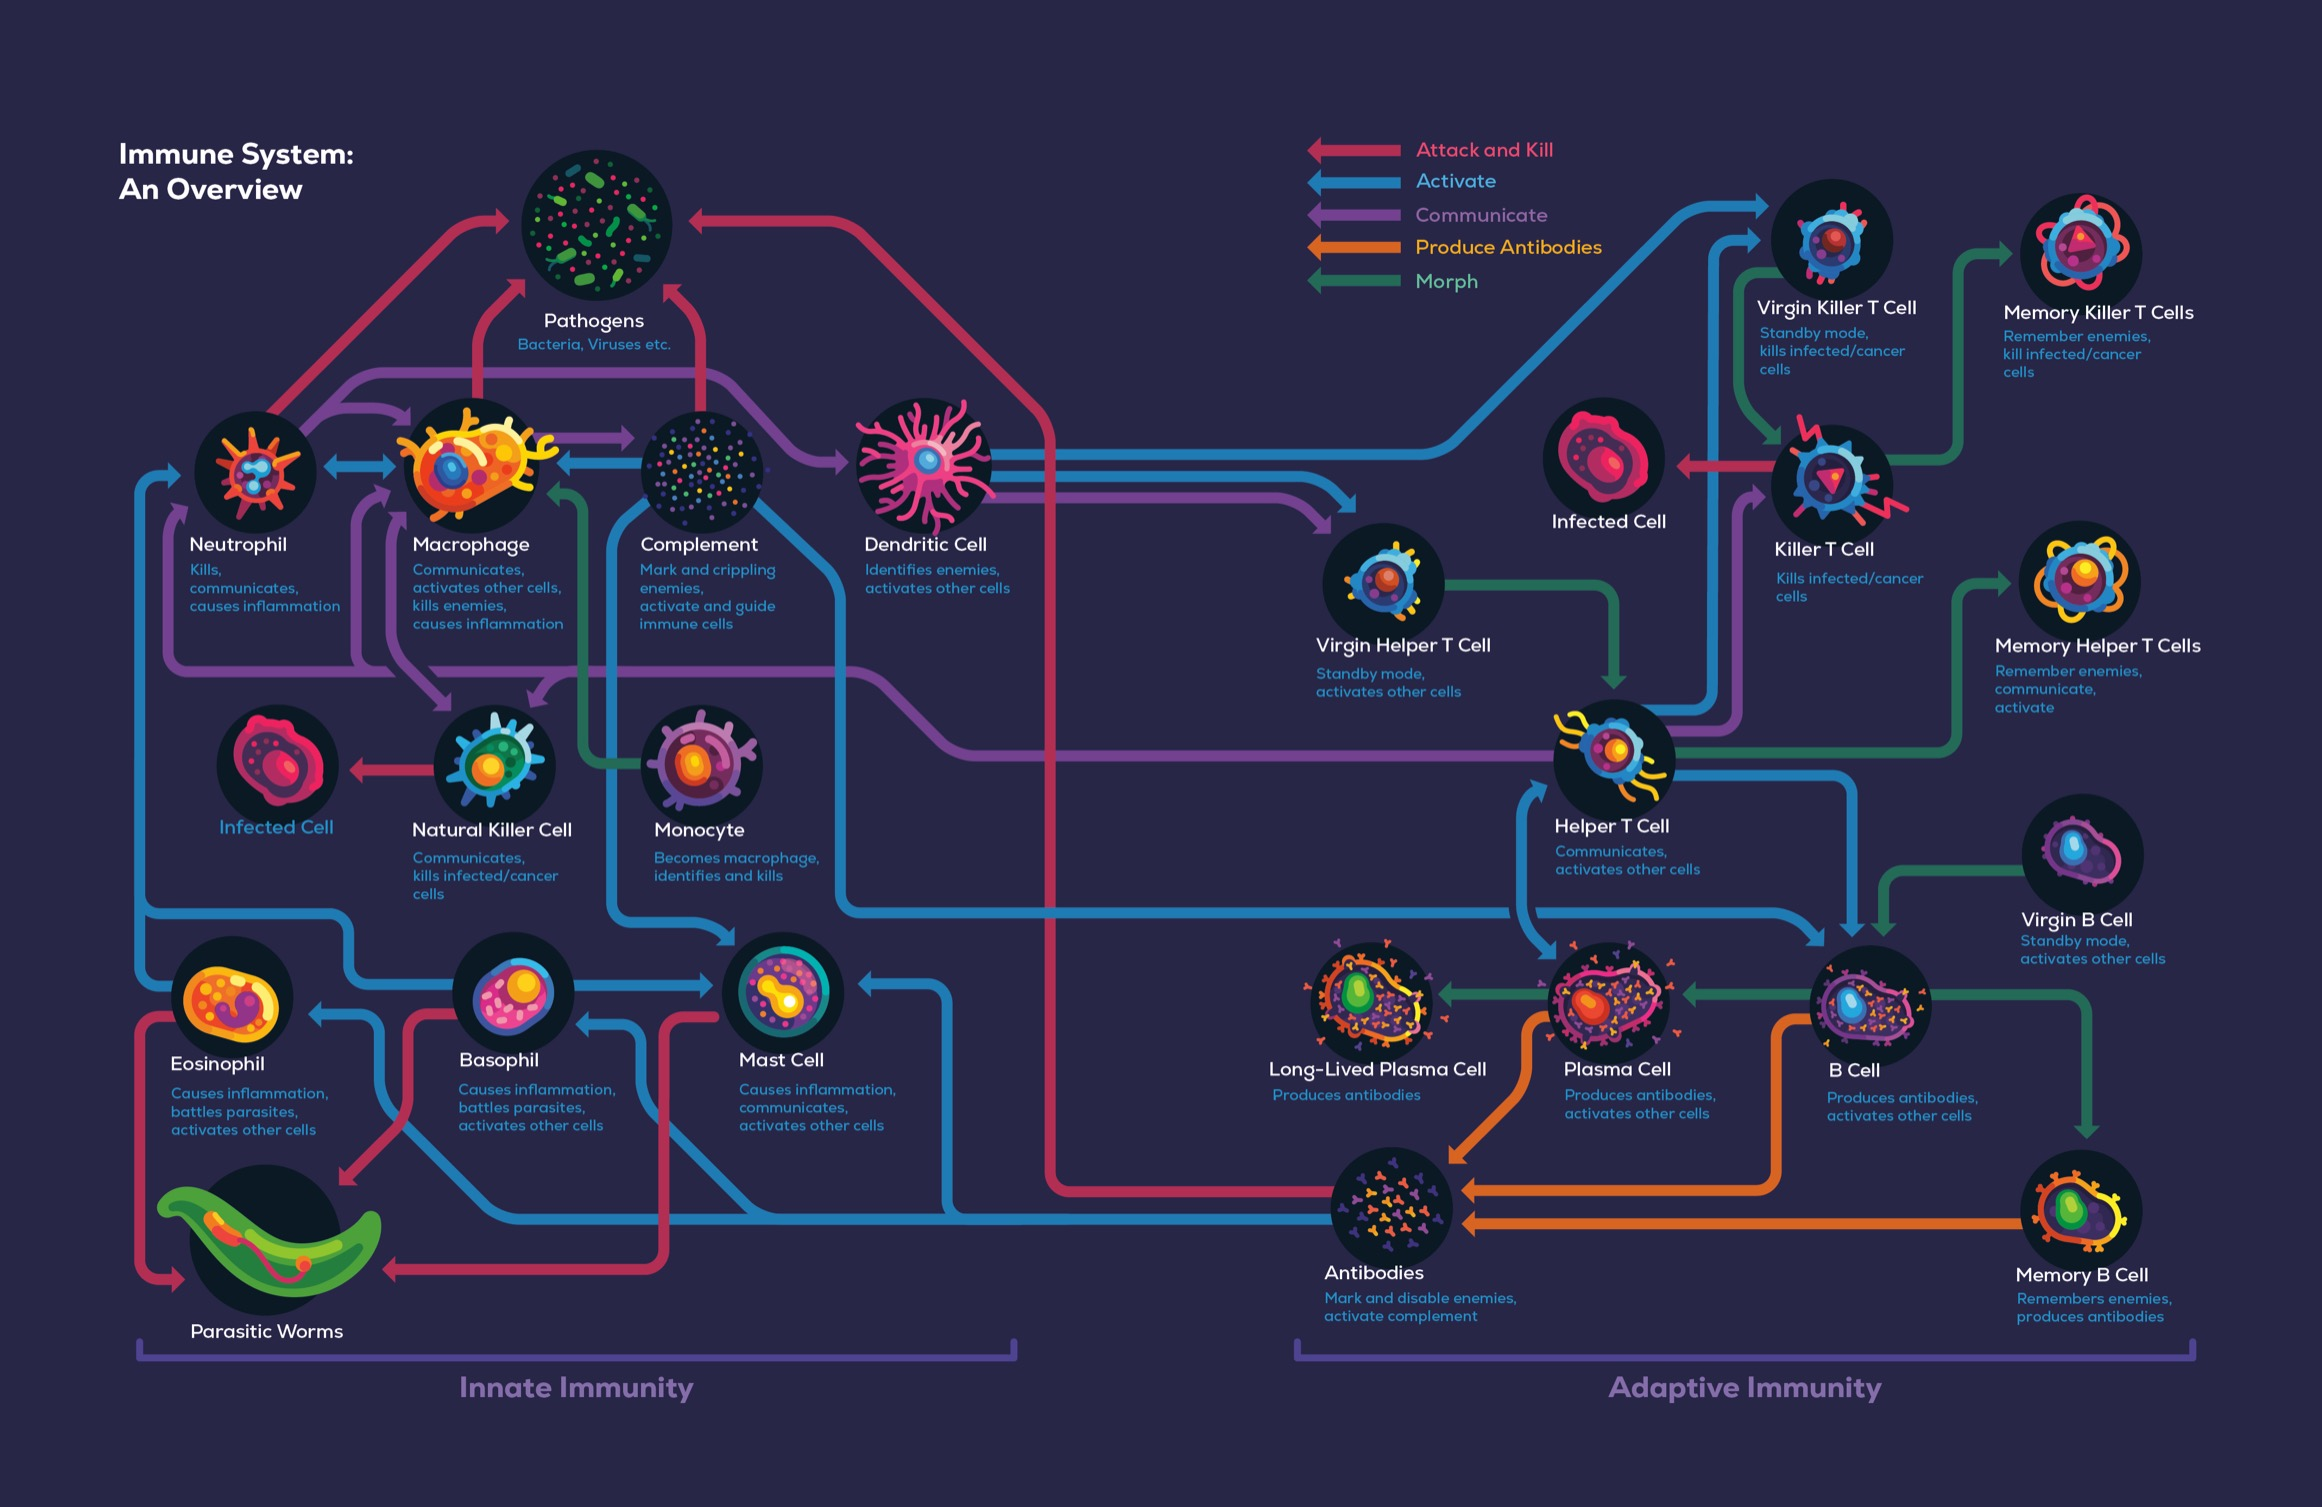
\includegraphics[scale=0.5]{figures/summary-immune-system.jpg}
    \caption[\textbf{An overview of the immune system}]{The red and the blue edges display direct cell-cell interactions, requiring ligand-receptor bound. On the contrary, the purple and orange edges characterise long-range interactions, through the release of respectively chemical signals or antibodies. Finally, the green edge depicts differentiation from one developmental stage to another for a given cell lineage. This figure is reproduced from \autocite[Figure 1, Chapter 42]{dettmer21}}. 
    \label{fig:summary-immune-system}
\end{figure}

In the next section, weinstead talk proficiently about the disorders of the immune system, when it is not anymore in its balanced operating order, and its strong consequences on the human health.

\subsection{Immune dysregulation}

While the immune system is essential to fend off pathogens or wipe out tumoral cells, the strength of the response, especially when occurring at the scale of the organism, results in  detrimental side effects. Hence, a heightened inflammatory response triggered by global tissue damage or blood contamination, is likely to lead to a life-threatening condition, called \emph{septic shock}. It is notably characterised by an increase by several folds of the number of white blood cells, a higher temperature resulting in \emph{fever} at the human organism scale and low blood pressure. We discuss of one of these exacerbated mechanisms in the context of \enquote{cytokine storms}, life-threatening events that occur among many patients overwhelmed by the Covid19 infection, in \Cref{sec:covid19-repurposing}. 

Additionally, not only pathogens can be recognised as non-self, but also any foreign molecule, even issued from other human bodies. The huge number of variations of the  MHC molecules \footnote{the MHC complex not only displays antigen fragments, but a subset of the proteins composing it, the Human leukocyte antigens (HLA) act as an identity card that asserts the immune system that the investigated cell belongs to self} between two individuals prompts transplants or grafts rejection. The only way to counterbalance rejection is to pair match the MHC molecules of the donor and the receptor as much as possible, and to use immuno-suppressor drugs.

A similar mechanism is involved in blood transfusions, but instead of the HLA complex, glycoproteins on the surface of red blood cells are recognised as foreign, eliciting lysis of the transferred blood cells, necrosia and kidney failure. For long, the only way to overcome this process was to control, prior to the transfusion, that the the patient and the donor had compatible blood groups (based on one of the two possible glycoproteins, A or B,  or absence of both of them, marked as O, knowing that patients could only receive blood cells with antigens already present in their organism).
\autocite{olsson_clausen08} reviews pioneering studies made in the development of enzymatic conversion of blood group A and B red blood cells to O for creating a universal blood supply. This includes the use of novel bacterial exoglycosidases with improved properties for cleaving A and B carbohydrates.


Nonetheless, all previous situations correspond to an expected behaviour of the immune system against foreigners, and it is either medicine progress or particularly virulent pathogens that trigger life-threatening conditions. However, the immune system can display aberrant behaviour, often elicited by a failure of the regulation mechanisms (see \Cref{subfig:immuno-vs-cancer} and \autocite{schnell_etal20}). Bad regulation of the immune system often come as the two sides of a coin: \emph{dysregulation} of the immune system leads to an over-activation of the immune system \autocite{rosenblum_etal15}, while \emph{misregulation}, an under-activation of the immune system plays a prominent role in the evolution of the cancer, acting as the prime actor of immune escape \autocite{chakraborty_etal22}. Although auto-inflammatory diseases are typically not fatal by themselves, they can severely compromise the health and well-being of afflicted patients. The Sjögren's syndrome, a condition upon which my attention was particularly focused  is studied in further details in \Cref{sec:sjogren-clustering}. Briefly, we display on \Cref{subfig:autoimmune-origin} below a possible causal factor that elicits the production of self-antigens, and the state-of-the-art parthenogenesis of one of the most common inflammatory ailment in \Cref{subfig:cross-reactivity}, namely sclerosis, best known for taking the life of Stephen Hawking.


\begin{figure}
     \centering
     \begin{subfigure}[p]{0.45\textwidth}
         \centering
         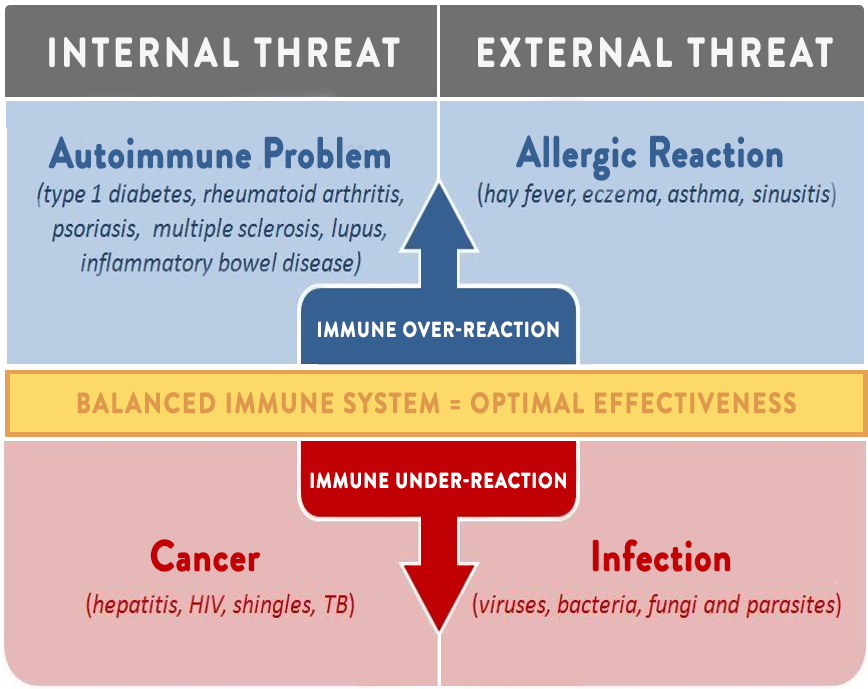
\includegraphics[width=\textwidth]{figures/immuno/The-Link-Between-Cancer-and-Autoimmune-Disease.jpg}
         \label{subfig:immuno-vs-cancer}
         \caption[\textbf{Autoimmune diseases and cancers: the two sides of the same coin.}]{Cancer and autoimmune diseases represent two distinct pathological states. Regarding cancer, the main mechanism involving immune cells is \textit{tumour escape}, in which the immune response is incapable of eliminating self-cells that have undergone transformation. Conversely, autoimmune diseases are characterised by an overactive immune response directed towards self-particles wrongly recognised as antigens, resulting in tissue damage and chronic inflammation. However, autoimmunity and cancer both hinge on a failure of the immune system in controlling abnormal cell proliferation (respectively auto-reactive immune cells or tumour cells). Furthermore, both ailments share analogous mechanistic immune responses, including the recruitment of phagocytes and neutrophils, as well as the activation of hypoxia and angiogenesis processes. Reproduced from \autocite[Fig .4]{sarah18}.}
     \end{subfigure}
     \hfill
     \begin{subfigure}[p]{0.45\textwidth}
         \centering
         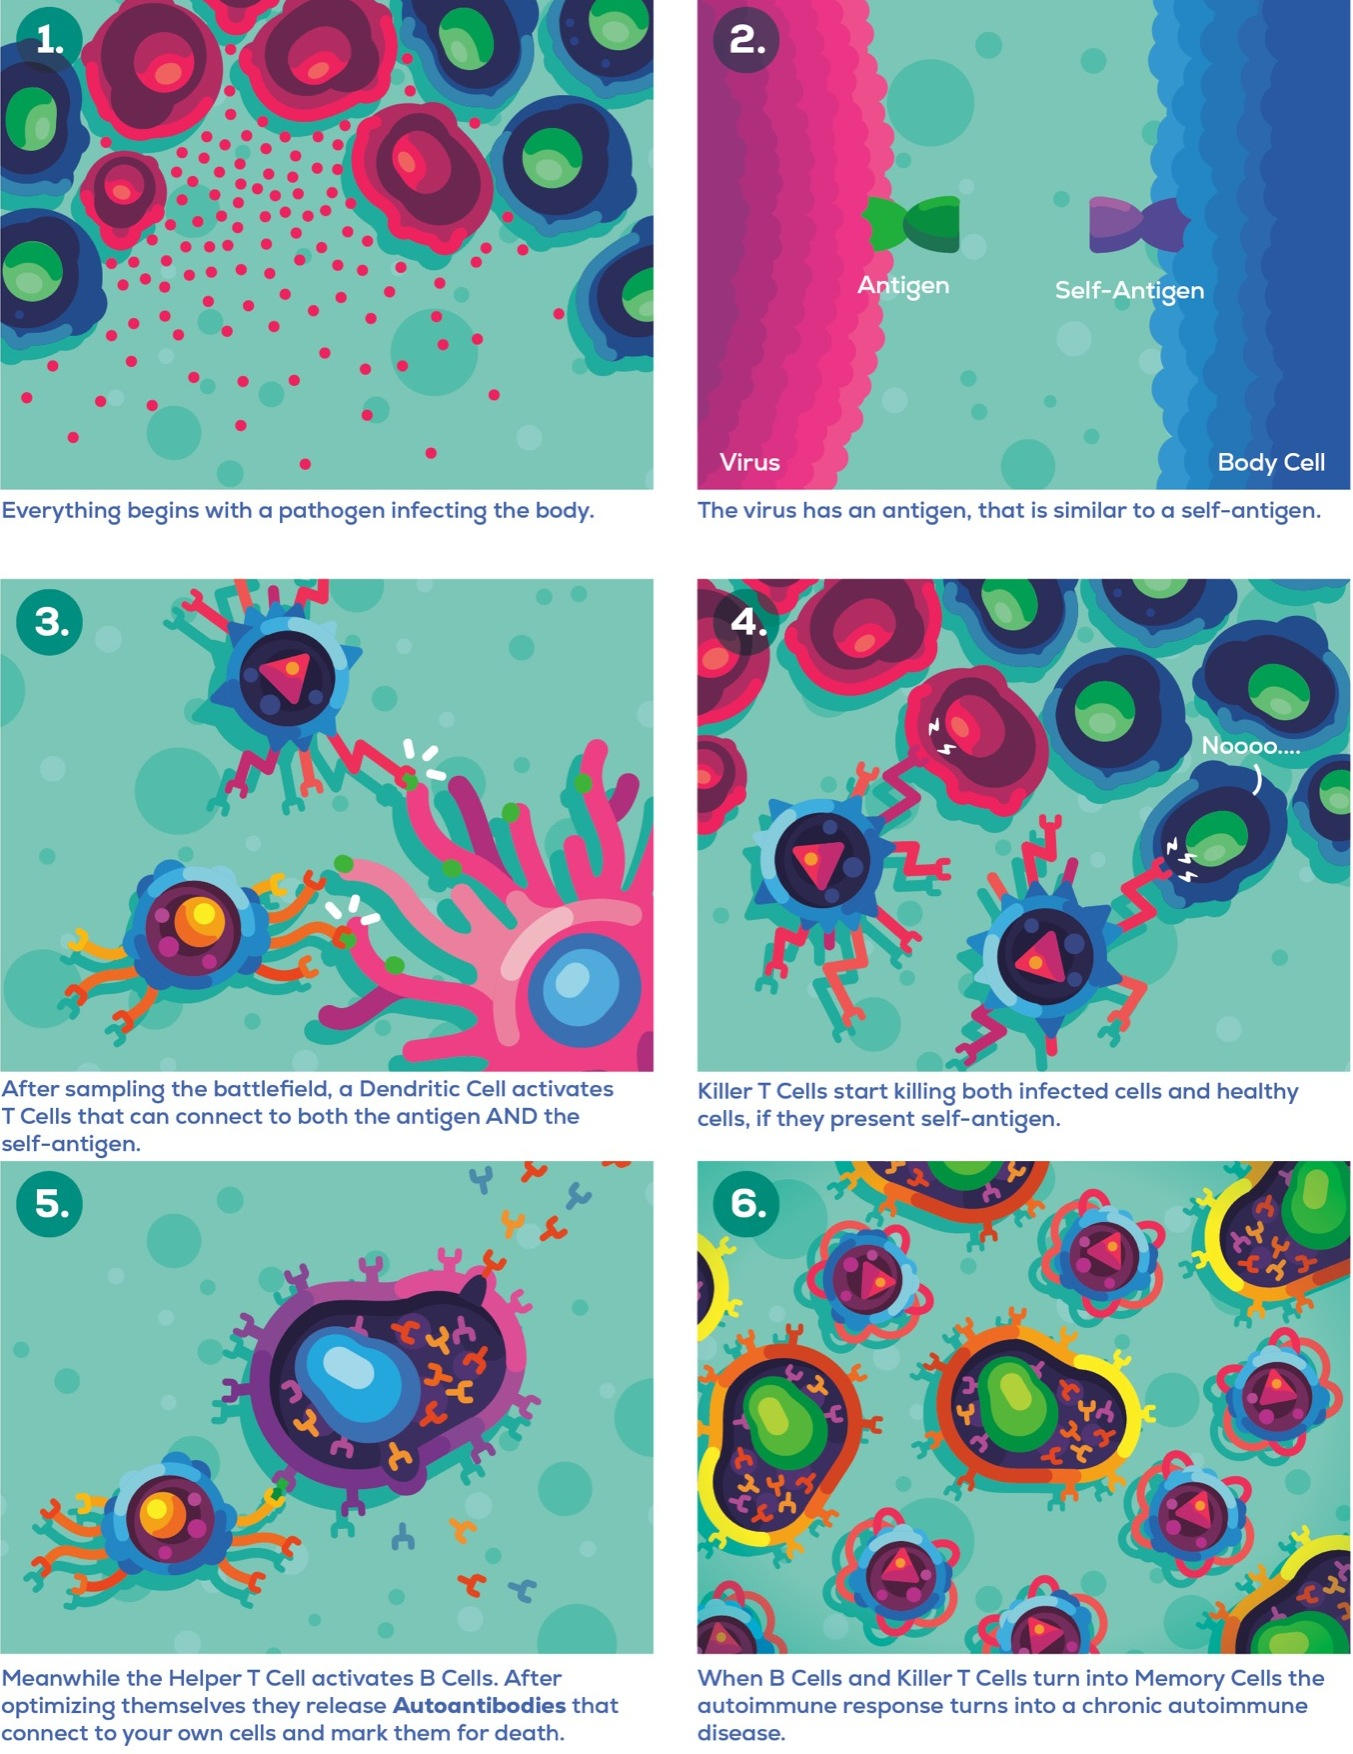
\includegraphics[width=\textwidth]{figures/immuno/kurzgesagt_autoimmune_origin.jpg}
         \label{subfig:autoimmune-origin}
         \caption[\textbf{Cross-reactivity, a prominent etiological factor in the initiation of autoimmune diseases.}]{Dysregulation at several layers of the immune system,  such as the complement system, interferon or cytokine production, can contribute to a variety of diseases, including autoimmune diseases (Crohn’s disease), inflammatory disorders, and infections, notably when the antigens hide from the immune system or when own molecules are recognised as non-self. One major etiological factor which may elicit the genesis of auto-immune diseases is the close proximity of the epitopes present in ubiquitous bacteria with fragments of endogenous molecules. Reproduced from \autocite[Fig. 1, Chap. 40]{dettmer21}.}
     \end{subfigure}
     \vfill
     \begin{subfigure}[p]{0.8\textwidth}
         \centering
         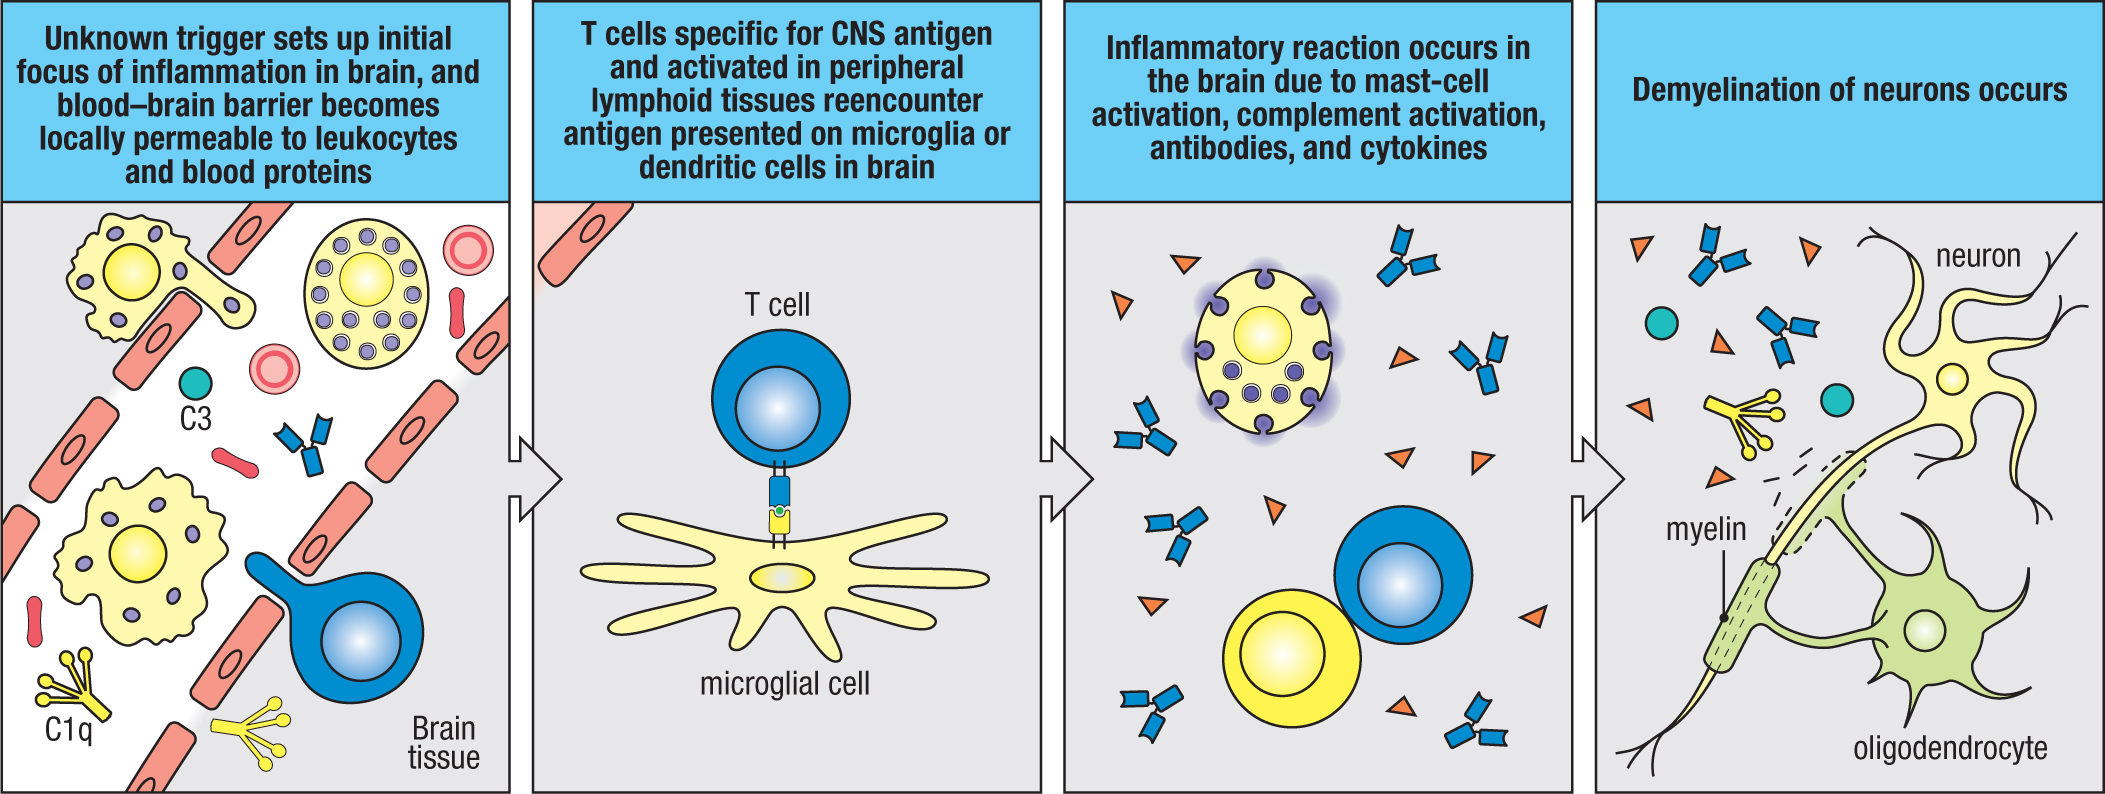
\includegraphics[width=\textwidth]{figures/immuno/cross_reactivity.jpg}
         \label{subfig:cross-reactivity}
         \caption[\textbf{The pathogenesis of multiple sclerosis (MS).}]{MS disease is among the affections studied in the Preciseads cohort \autocite{soret_etal21} \autocite{barturen_etal21}, a large European initiative aimed at deciphering the mechanisms involved in five systemic autoimmune diseases. It is also one of the three inflammatory illnesses, commensurate with those tailored for Sjögren's disease and Systemic Lupus Erythematosus (SLE). The objective is to release within five years promising groundbreaking treatments (see \Cref{sec:sjogren-clustering} for details). While the precise etiology of MS remains elusive, however, the immune mechanics involved afterwards are relatively clear. In inflamed regions, autoreactive T cells  infiltrate the brain through the blood-brain barrier and target brain antigens displayed on microglial cells. Upon contact, they secrete cytokines including, but not limited to IFN-$\gamma$, which in turn further enhance inflammation by chemio-attracting additional cells and complement proteins. Reproduced from \autocite[Fig. 15.25, Chap. 25]{murphy_etal22}.}
     \end{subfigure}
\end{figure}


In conclusion, it is important to recall from the previous section that the immune system is an intricate and interconnected network of cell populations and cytokines interplaying altogether to safeguard the body against foreign invaders. However, even a slight disruption in one of these mechanisms can result in a potentially life-threatening condition. For example, an overstimulation of T and B cells can lead to the development of an autoimmune disease, wherein the body begins to attack its own cells. On the other hand, an over-activation of the regulatory system can result in chronic infections, similar to those observed in patients with AIDS, or the unabated proliferation of malignant tumours.
	Related with auto-immune subjects, and having personally to debate with my acknowledges on the hypothetical benefits of alternative therapies over complex, costly treatments designed by pharmaceutical companies, you should never fall for the miracle effects claimed by the supplement industry, above all from the homeotherapy branch. To quote the author of the \texttt{Kurzgesagt – In a Nutshell initiative}, \autocite{dettmer21}: 
	\begin{displayquote}
	At least for now, there are no scientifically proven ways to directly boost your immune system with any products that are easily available. And if there were, it would be very dangerous to use them without medical supervision.
	\end{displayquote}
	 Indeed, the assertion of enhancing the immune system is predicated on the notion that a balanced immune system is preferable to a robust but unguided one. In reality, the process of recalibrating the crosstalk between the components of the immune system to restore homoeostasis is challenging, highly specific to the disease, and impervious to any panacea or cure-all substance.
	



%\subsubsection{Auto-immune diseases}
%\label{subsec:auto-immune disease}



%\subsubsection{Immunology-oncology}
%\paragraph{Overview: the hallmarks of cancer}
%\paragraph{Pro and anti-tumoral environments}
%\todo[fancyline]{The tumoral micro environment, the text below refers methods from \autocite{longo_etal21}}
%Although spatial transcriptomics analyses of several disease microenvironments exist, tumour microenvironments are presently the most extensively studied46. Tumour microenvironments are particularly heterogeneous and have complex, spatially restricted interactions with the immune system47,48. Until recently, the ability to interrogate the inner workings and heterogeneity of the tumour microenvironment has relied largely on bulk RNA-seq49. scRNA-seq has advanced our understanding by identifying cancer subpopulations that can drive drug resistance, predict metastatic risk and provide prognostic value50,51.
%A recent study combined spatial barcoding and scRNA-seq to localize an immunosuppressive tumour-specific keratinocyte subpopulation to a fibrovascular niche at the tumour borders (as defined by aligning haematoxylin and eosin images) in human squamous cell carcinoma33. This population expressed genes associated with immunotherapy resistance and numerous ligands inferred to modulate cancer-associated fibroblasts, suggesting ways tumour subpopulations may promote local immunosuppression. In pancreatic ductal adenocarcinoma, another study intersected scRNA-seq and spatial barcoding with annotated haematoxylin and eosin images to reveal that inflammatory fibroblasts play a significant role in cancer stress responses34. In addition to providing insights into tumour resistance and stress responses, such integrated data may offer insight into clinical prognosis. For example, one study observed that greater heterogeneity of a transition area within cross-sections of melanoma metastases was associated with poorer patient survival35. Furthermore, spatial data enabled the identification of the most abundantly expressed genes in the transition area
%\todo{Hétérogénéité tumorale et plasticité dans l’espace et le temps, conférence (et aussi pour le TME)}
%
%\paragraph{Monoclonal treatments}
%
%However, cultivated monoclonal antibodies are issued
%from the same ancestral B cell and amplified through multiple division cycles. Monoclonal
%antibodies are also being used as therapies
%for a growing number of human diseases,
%including many cancers.
%
%













